\documentclass[edeposit,fullpage,11pt]{uiucecethesis09}
% Use draftthesis for notes and date markings on every page.  Useful when you
%   have multiple copies floating around.
% Use offcenter for the extra .5 inch on the left side. Needed with fullpage and fancy.
% Use mixcasechap for compatibility with hyperref package, which does NOT like all caps default
% Use edeposit for the adviser/committee on the title page.
% Use tocnosub to suppress subsection and lower entries in the TOC.
% PhD candidates use "proquest" for the proquest abstract.

\makeatletter

\usepackage{setspace}
%\usepackage{epsfig}  % for figures
\usepackage{graphicx}  % another package that works for figures
\usepackage{multirow}
\usepackage{placeins}
\usepackage{caption}  % allows center figures caption
\usepackage{booktabs} % nice rules (thick lines) for tables
\usepackage{array}
\usepackage{tabularx}
\usepackage[table]{xcolor}
\newcolumntype{b}{>{\hsize=1.0\hsize}X}
\newcolumntype{s}{>{\hsize=.5\hsize}X}
\newcolumntype{m}{>{\hsize=.75\hsize}X}
\newcolumntype{x}{>{\hsize=.25\hsize}X}
\newcolumntype{L}{>{\raggedright\arraybackslash}X}
\newcolumntype{R}{>{\raggedleft\arraybackslash}X}
\def\arraystretch{1}
\graphicspath{{figures/}}
%\usepackage{subfigure}  % for subfigures
\usepackage{amsmath}  % for math spacing
%\usepackage{amssymb}  % for math spacing
%\usepackage{url}  % Hyphenation of URLs.
\usepackage{lscape}  % Useful for wide tables or figures.
\usepackage[justification=raggedright]{caption}	% makes captions ragged right - thanks to Bryce Lobdell
\usepackage[acronym,toc]{glossaries}  % acronyms inclusion
\usepackage{color,soul}
\makeglossary
\usepackage{xspace}
\usepackage{float}
\usepackage{subcaption}
\newcommand{\Cyclus}{\textsc{Cyclus}\xspace}%
\newcommand{\Cycamore}{\textsc{Cycamore}\xspace}%
\newcommand{\deploy}{\texttt{d3ploy}\xspace}%

\usepackage{amsmath}%
\usepackage{MnSymbol}%
\usepackage{wasysym}%

\usepackage{tikz}
\usetikzlibrary{positioning, arrows, decorations, shapes}
\usetikzlibrary{shapes.geometric,arrows}

\definecolor{illiniblue}{HTML}{B1C6E2}
\definecolor{illiniorange}{HTML}{f8c2a2}
\usetikzlibrary{shapes.geometric, arrows}
\tikzstyle{oblock} = [rectangle, draw, fill=illiniorange, 
text width=15em, text centered, rounded corners, minimum height=4em]
\tikzstyle{bblock} = [rectangle, draw, fill=illiniblue, 
text width=15em, text centered, rounded corners, minimum height=4em]
\tikzstyle{sbblock} = [rectangle, draw, fill=illiniblue, 
text width=15em, text centered, rounded corners, minimum height=4em]
\tikzstyle{arrow} = [thick,->,>=stealth]
\tikzstyle{sbblock} = [rectangle, draw, fill=illiniblue, 
text width=7em, text centered, rounded corners, minimum height=4em]


% Uncomment the appropriate one of the following four lines:
\msthesis
%\phdthesis
%\otherdoctorate[abbrev]{Title of Degree}
%\othermasters[abbrev]{Title of Degree}

\title{Gwen Thesis}
\author{Gwendolyn J. Chee}
\department{Nuclear, Plasma, and Radiological Engineering}
\degreeyear{2019}

% Advisor name is required for
% - doctoral students for the ProQuest abstract
% - master's students who do not have a master's committee
%\advisor{Professor Kathryn D. Huff}

% Uncomment the \committee command for
% - all doctoral students
% - master's students who have a master's committee
\committee{Assistant Professor Kathryn Huff, Chair\\
           who knows} % etc.

\begin{document}
\include{acros}
%%%%%%%%%%%%%%%%%%%%%%%%%%%%%%%%%%%%%%%%%%%%%%%%%%%%%%%%%%%%%%%%%%%%%%%%%%%%%%%
% TITLE
%
\maketitle

%\raggedright
\parindent 1em%

\frontmatter

%%%%%%%%%%%%%%%%%%%%%%%%%%%%%%%%%%%%%%%%%%%%%%%%%%%%%%%%%%%%%%%%%%%%%%%%%%%%%%%
% ABSTRACT
%
\begin{abstract}
% Put the abstract in a file called "abs.tex" and it'll be inputted here.
\vspace{-1.5cm}
The present United States nuclear fuel cycle faces challenges that hinder 
the expansion of nuclear energy technology. 
The U.S. Department of Energy identified four nuclear fuel cycle 
options we could transition to, which would overcome these challenges 
and make nuclear energy technology more desirable. 
In this work, our first goal is to model the transition from our current
state to a promising future end-state.
In reality, the real transition process inevitably diverges from the 
modeled scenario. 
Therefore, our second goal is to conduct sensitivity analysis 
studies to understand the impact changes in technology deployment 
strategies have on the transition. 
Accordingly, we developed demand-driven deployment capabilities 
(\deploy) in Cyclus, a nuclear fuel cycle simulator. 
\deploy predictively and automatically deploys fuel cycle facilities 
to meet user-defined power demand.
We demonstrated \deploy's capability to automatically deploy fuel 
cycle facilities to set up a transition scenario from the current 
fleet to a combination of mixed oxide fuel pressurized water reactors 
and sodium fast-cooled reactors. 
In this work, we coupled nuclear fuel cycle simulators, DYMOND 
and \Cyclus, with Dakota, a sensitivity analysis tool. 
We demonstrated 
one-at-a-time, synergistic, and global sensitivity analysis studies.
We compared DYMOND and \Cyclus' sensitivity analysis capabilities 
and concluded that automated deployment of supporting fuel cycle 
facilities is crucial for conducting sensitivity analysis studies 
with nuclear fuel cycle simulators, to ensure that the simulation 
adapts to the new parameters by minimizing idle reactor capacity. 
We recommend that a comprehensive sensitivity analysis of a 
nuclear fuel cycle transition scenario begin with a global 
sensitivity analysis study to gain a general overview of the 
influential input variables for the performance metrics. 
Using the global sensitivity analysis results, 
conduct one-at-a-time and synergistic sensitivity 
analysis to determine quantitative trends and impacts of influential 
input variables on the performance metrics.

\end{abstract}

%%%%%%%%%%%%%%%%%%%%%%%%%%%%%%%%%%%%%%%%%%%%%%%%%%%%%%%%%%%%%%%%%%%%%%%%%%%%%%%
% DEDICATION
%
\begin{dedication}
dedication
\end{dedication}

%%%%%%%%%%%%%%%%%%%%%%%%%%%%%%%%%%%%%%%%%%%%%%%%%%%%%%%%%%%%%%%%%%%%%%%%%%%%%%%
% ACKNOWLEDGMENTS
%
% Put acknowledgments in a file called "ack.tex" and it'll be inputted here.
\begin{acknowledgments}
I want to express my deepest gratitude to my advisor, 
Dr. Kathryn Huff, for her guidance, patience, and 
support in my learning journey towards becoming a proper scientist.
I also wish to thank Dr. Bo Feng from Argonne National 
Laboratory for his guidance and direction in conducting 
sensitivity analysis studies and invaluable career advice.  
I would also like to acknowledge Dr. James Stubbins as the 
second reader of this thesis; I am grateful for his valuable 
comments on this thesis. 
This work would not have been possible without the 
financial support of the Nuclear Energy University Program 
for funding me through (Project 16-10512, DE-NE0008567) 
`Demand-Driven Cycamore Archetypes'.

I thank my fellow groupmates, for the embodiment of `misery 
loves company', Greg Westphal, Jin Whan Bae, Sun Myung Park, 
Roberto Fairhurst, Anshuman Chaube, Kip Kleimenhagen, 
Gyu Tae Park, Andrei Rykhlevskii, and Sam Dotson. 
Special thanks to Kip Kleimenhagen for his excellent proofreading. 
I also had the pleasure of collaborating with the wonderful 
and supportive Cyclus community, particularly those in the 
University of Wisconsin \gls{CNERG} and the University of 
South Carolina Energy Research Group (ERGS). 
I am also grateful to my WiN family for my weekly dose 
of good vibes and rapport. 
Special thanks to my roommate, Mao, who always brightened my 
day with baked goods and funny memes. 

Finally, I cannot begin to express my thanks to my parents, 
Joy and Gerard, and my brother, Ben, for their unwavering love 
and support from day one. 


\end{acknowledgments}																																				
%%%%%%%%%%%%%%%%%%%%%%%%%%%%%%%%%%%%%%%%%%%%%%%%%%%%%%%%%%%%%%%%%%%%%%%%%%%%%%%
% TABLE OF CONTENTS
%
\tableofcontents

%%%%%%%%%%%%%%%%%%%%%%%%%%%%%%%%%%%%%%%%%%%%%%%%%%%%%%%%%%%%%%%%%%%%%%%%%%%%%%%
% LIST OF TABLES
%
% The List of Tables is not strictly necessary. Omitting the List of Tables will
% simplify the thesis check and reduce the number of corrections.
\listoftables

%%%%%%%%%%%%%%%%%%%%%%%%%%%%%%%%%%%%%%%%%%%%%%%%%%%%%%%%%%%%%%%%%%%%%%%%%%%%%%%
% LIST OF FIGURES
%
% The List of Figures is not strictly necessary. Omitting the List of Figures will
% simplify the thesis check and reduce the number of corrections.
\listoffigures

%%%%%%%%%%%%%%%%%%%%%%%%%%%%%%%%%%%%%%%%%%%%%%%%%%%%%%%%%%%%%%%%%%%%%%%%%%%%%%%
% LIST OF ABBREVIATIONS
%
% The List of Abbreviations is not strictly necessary.
%\chapter{LIST OF ABBREVIATIONS}

%\printacronyms
%\begin{symbollist*}
%\item[MSBR] Molten Salt Breeder Reactor
%\item[MSR] Molten Salt Reactor
%\item[ORNL] Oak Ridge National Laboratory
%\end{symbollist*}


%%%%%%%%%%%%%%%%%%%%%%%%%%%%%%%%%%%%%%%%%%%%%%%%%%%%%%%%%%%%%%%%%%%%%%%%%%%%%%%
% LIST OF SYMBOLS
%
%\begin{symbollist}[0.7in]
%\item[$\tau$] Time taken to drink one cup of coffee.
%\end{symbollist}

\mainmatter

%%%%%%%%%%%%%%%%%%%%%%%%%%%%%%%%%%%%%%%%%%%%%%%%%%%%%%%%%%%%%%%%%%%%%%%%%%%%%%%
% INSERT REAL CONTENT HERE
%
\chapter[Introduction]{Introduction}

\section{Background and motivation}
\subsection{Why is Nuclear Waste Disposal research important?}
Implementation of a nuclear waste disposal plan and minimizing the 
cost of the nuclear fuel cycle are crucial to the future use of 
nuclear power 
\cite{massachusetts_institute_of_technology_future_2003}. 
If the U.S. nuclear industry does not find an effective and safe 
plan to manage the waste, the nuclear industry will continue facing 
political and social opposition. 

[**More]

\subsection{Possible Methods of Waste disposal}
Currently, all of the commercial nuclear waste in the \gls{US} are 
scattered across the country at each reactor site [** Reference]. 
There has been much debate on what to do with the nuclear waste in 
the long term. 
There has been much debate between an open fuel cycle and a closed 
fuel cycle. 

[**Describe Open Fuel Cycle]

[**Describe Closed Fuel Cycle, why does France use it?]

[**Compare them -- advantages and disadvantages of each]

[**Describe why an open fuel cycle is more feasible in the US]
It was determined in the large multi-disciplinary study of the 
future of nuclear power that a once-through fuel cycle is more 
economic and proliferation-resistant than a closed fuel cycle that
makes use of reprocessing technology
\cite{massachusetts_institute_of_technology_future_2003}.

[**Waste Repository is necessary no matter what because every 
fuel cycle will have non-reprocessable waste]

In this work, the expectation is that the chosen fuel cycle is a 
once through fuel cycle and the method of long term disposal of 
spent nuclear fuel (SNF) will be a deep geologic repository. 

\subsection{Previous Work towards repository modeling}
Previous work towards the wicked problem of getting spent nuclear fuel from reactor 
sites to a final waste repository focuses on how different waste acceptance strategies 
impact economic expenditure \cite{nesbit_proposed_2015}, pre-emplacement 
surface storage time, waste package size, and repository 
footprint \cite{greenberg_application_2012}. 
There has also been efforts to holistically evaluate the entire system to consolidate 
how each factor impact the cost and safety of moving SNF from 
reactor sites to the final waste repository \cite{nutt_waste_2015}.
Previous work in studying repository loading have used spent fuel assemblies 
that have an average burn up composition \cite{johnson_optimizing_2016} 
to evaluate the heat load in the repository \cite{greenberg_application_2012}. 

\section{Objectives}
The objective of this thesis is to: 
\begin{itemize}
    \item Create a \Cyclus spent fuel conditioning model that
    packages spent fuel bundles into packages which have
    user-defined properties.
    \item Create a \Cyclus interim storage facility that gives 
    waste canisters to the repository facility to emplace in the 
    order of a specific waste acceptance strategy. 
    \item Create a \Cyclus medium-fidelity repository model that
    accepts and emplaces canisters that results in the repository 
    remaining below the thermal limit of the host geologic media.
    It should also give accurate time and spatial dependent 
    temperature values in the repository. 
    \item Use U.S. historical SNF inventory data 
    \cite{peterson_unf-st&dards_2017} in various simulations
    that model different loading strategies for moving 
    \gls{SNF} from reactor sites to a final waste repository.
\end{itemize}


\section{Methods}
Explain \Cyclus, \Cycamore, \Cyder etc.  	% for INTRODUCTION in "intro.tex"
\chapter[chapter 2]{Literature Review}

\section{History of Nuclear Fuel Cycle Simulators}
% What is a nuclear fuel cycle
The \gls{NFC} represents the life cycle of nuclear fuel from initial
extraction, processing, use in reactors, and eventually to 
final disposal.
It is a complex system of facilities and mass flows 
that are combined to meet the goal of providing nuclear energy 
in the 
form of electricity \cite{yacout_modeling_2005}.
An open \gls{NFC} is if used fuel is not reprocessed and a 
closed \gls{NFC} is if used fuel is reprocessed. 
Presently, the \gls{US} has an open \gls{NFC}. 
Whereas, an example of a country that has a 
closed \gls{NFC} is France. 

% Purpose of NFCSims 
\glspl{NFCSim} are system analysis tools used to evaluate 
quantitative measures of performance related to the dynamics of 
a \gls{NFC} on both high and low resolution. 
An example of a high-resolution element is the plutonium 
concentration in a single used fuel bundle, and an example 
of a low-resolution element is total electricity produced. 
The purpose of \glspl{NFCSim} is to better understand the 
dependence between various input parameters and components 
in the \gls{NFC} system and the impact of their variations on 
the system's performance. 
The results of \glspl{NFCSim} are being used to guide research 
efforts, advise future design choices and to provide 
decision makers with a transparent tool for evaluating \glspl{FCO} 
to inform big-picture policy decisions \cite{yacout_modeling_2005}.

% Where are NFC codes from 
Historically, international national laboratories have driven 
development and are the major users of \gls{NFCSim} tools. 
However, due to propriety access to these tools, universities and 
other non-laboratory organizations have taken to creating their 
own tools. 
Table \ref{tab:nfctools} shows a breakdown of the \glspl{NFCSim}
and the organization(s) associated with it. 

\begin{table}[]
    \centering
    \resizebox{0.7\textwidth}{!}{%
    \begin{tabular}{|l|l|}
    \hline
    \textbf{\gls{NFCSim}} & \textbf{Organization(s) associated with it}                                    \\ \hline
    \Cyclus \cite{huff_fundamental_2016}                & \begin{tabular}[c]{@{}l@{}}\gls{UW} \\ \gls{UIUC}\end{tabular} \\ \hline
    DYMOND \cite{yacout_modeling_2005},                                & \gls{ANL}                                                                                               \\ \hline
    ORION  \cite{gregg_analysis_2012}                                & \gls{NNL}                                                                                             \\ \hline
    VISION \cite{jacobson_vision:_2006}                                & \gls{INL}                                                                                               \\ \hline
    COSI   \cite{coquelet-pascal_cosi6:_2015}                                &   \gls{CEA}                    \\ \hline
    CLASS  \cite{mouginot_class_2012}                                &  \begin{tabular}[c]{@{}l@{}}\gls{CNRS} \\ \gls{IRSN}\end{tabular}                                      \\ \hline
    DESAE  & \gls{OECD} \\ \hline
    \end{tabular}%
    }
    \caption{Nuclear Fuel Cycle Simulator Tools and their corresponding organizations.}
    \label{tab:nfctools}
    \end{table}

% what is agent, what is fleet
One of the major distinctions between the various \glspl{NFCSim}
is fleet-level or agent-level modeling of facilities and materials. 
Fleet-based models do not distinguish between discrete facilities 
or materials, but instead lump them together into fleets and streams. 
The advantages of this method is a simpler code structure and 
lower computational cost. 
Agent-based models treats facilities and materials as discrete 
objects. 
The advantages of this method are more flexible simulation control
and ease of simulating a wide range of scenarios with new 
technologies.  

% why is it good that there are multiple tools 
% benchmark against each other
Efforts have been made towards benchmarking \gls{NFCSim} 
tools against each other to verify them 
\cite{feng_standardized_2016,guerin_benchmark_2009}. 
These comparison studies assist developers in modifying the
codes to more realistically model the \gls{NFC}. 
Also, by upholding the \gls{NFCSim} tools to high level agreement, 
stakeholders and decision makers can have more confidence in 
prediction results generated by \gls{NFCSim} tools and trust them 
to inform on potential strategic and policy decisions
\cite{feng_standardized_2016}. 

\section{Transition Scenarios}
In Chapter \ref{chap:1}, the history and motivation of
\gls{NFC} transition scenario research was described.
More detail about transition scenario studies will be given 
in this section. 

The evaluation and screening study identified 40 promising 
\glspl{EG} to represent a comprehensive set of 
\gls{FCO} \cite{wigeland_nuclear_2014}. 
To access the performance of each \gls{EG}, the study
used 9 evaluation criteria: nuclear waste management, 
proliferation risk, nuclear material security risk, 
safety, environmental impact, resource utilization, 
development and deployment risk, institutional issues, and 
financial risk.  
The conclusion of the study is that fuel cycles
involving continuous recycling of co-extracted U/Pu or U/TRU in 
fast spectrum critical reactors consistently scored high overall 
performance.
In the study, these fuel cycles were referred to as EG23, EG24, 
EG29 and EG30. 
Table \ref{tab:eg} provides a description of the current 
\gls{US} \gls{EG} and the promising \glspl{EG}. 
These \glspl{EG} were evaluated at an equilibrium state to 
understand the end-state benefits of each evaluation group (EG).
Knowing the most promising end state \glspl{EG}, 
the next step is to evaluate and compare the transition process 
from the current EG01 
state to the these \glspl{EG} \cite{feng_standardized_2016}. 

\begin{table}[]
	\centering
    \begin{tabular}{|l|l|}
        \hline
        Fuel Cycle & Description                                                                                                                                 \\ \hline
        EG01 (current)      & \begin{tabular}[c]{@{}l@{}}Once-through using enriched-U fuel in \\ thermal critical reactors.\end{tabular}                                 \\ \hline
        EG23       & \begin{tabular}[c]{@{}l@{}}Continuous recycle of U/Pu with new\\ natural-U fuel in fast critical reactors.\end{tabular}                     \\ \hline
        EG24       & \begin{tabular}[c]{@{}l@{}}Continuous recycle of U/TRU with new\\ natural-U fuel in fast critical reactors.\end{tabular}                    \\ \hline
        EG29       & \begin{tabular}[c]{@{}l@{}}Continuous recycle of U/Pu with new\\ natural-U fuel in both fast and thermal\\ critical reactors.\end{tabular}  \\ \hline
        EG30       & \begin{tabular}[c]{@{}l@{}}Continuous recycle of U/TRU with new\\ natural-U fuel in both fast and thermal\\ critical reactors.\end{tabular} \\ \hline
    \end{tabular}
    \caption{Descriptions of the current and other high performing nuclear fuel cycle evaluation groups described in the evaluation and screening study \cite{wigeland_nuclear_2014}.}
    \label{tab:eg}
\end{table}


\section{\glspl{NFCSim} Transition Scenario Capabilities}
% what has been done for transition scenarios so far
Both \gls{NFCSim} tools used in this thesis, \Cyclus and Dymond,
were verified by a benchmarking effort for use of 
\gls{NFCSim} tools to conduct transition scenario analyses
\cite{feng_standardized_2016,bae_standardized_2019}.
The reference problem used in the benchmark was a simplified 
transition of one hundred 1000-MWe \glspl{LWR} to a fleet 
of 333.3-MWe \gls{SFR} fleet. 
They were found to have excellent agreement with the 
spreadsheet solution and other \gls{NFC} codes.  
This benchmarking effort proved that these \glspl{NFCSim}
are capable of simulating a simple transition scenario. 
However, it acknowledged that there needs to be more efforts 
to model realistic transition scenarios to evaluate the
flexibility of the \glspl{NFCSim} \cite{feng_standardized_2016}.

% brown paper 
% teddy thesis for cyclus capabilties 

\section{\glspl{NFCSim} Sensitivity Analysis}
% SA for NFCs vs SA for NFC transition scenarios 

To enable \glspl{NFCSim} to produce insightful and 
flexible results to inform policy decisions, it is necessary 
to be able to quantify and include all the different aspects and 
subtleties of each segment of the \gls{NFC} through system analysis 
and sensitivity studies \cite{passerini_systematic_2014}. 
Previous work towards \gls{SA} and \gls{UQ} of \gls{NFC} 
simulations used them interchangeably. 
This is because \gls{UQ} in \glspl{NFCSim} are seen as design 
uncertainties. 
For example, a pyrochemical reprocessing facility has never been 
built, therefore, its throughput is viewed as a design parameter 
that can be varied. 
By conducting \gls{SA}/\gls{UQ} on the throughput design 
parameter, the impact on important output parameters can be 
determined. 
By conducting similar studies on a large set of input parameters, 
it will indicate which parameters have large impacts, giving a clear 
picture of where a closer sensitivity study should be conducted and 
where additional modeling detail should be added. 
It will also identify which parameters the system is relatively 
insensitive to \cite{noauthor_effects_2017}. 

\gls{SA} is a technique used to determine how 
varying input variable(s) will impact
output variables for a given scenario. 
Many assumptions are made when setting up the simulation scenarios, 
therefore, \gls{SA} will assist in the evaluation of
sensitivity of the output of the scenario to each of these 
assumptions.  
There are two types of sensitivity analysis: one-at-a-time (OAT)
and synergistic. 

OAT is basic \gls{SA} that focuses on estimating the lone effect 
of one input variable. 
This approach gives the local effect of each variable on the 
output parameters of interest. 
OECD conducted a OAT sensitivity analysis \cite{noauthor_effects_2017} 
on key \gls{NFC} input parameters
and quantified the impacts on the selected output parameters. 
They varied each parameter independently and expressed the effects 
on the output parameters in tornado plots and sensitivity tables. 
Figure \ref{fig:oecd-sensitivitytable} shows the sensitivity table
provided by the benchmark that gives an overview of their analysis. 
Figure \ref{fig:oecd-tornado} shows an example tornado plot that represents 
the sensitivity of separated Pu in storage to the various input parameters. 
% explain each figure more 


\begin{figure}[]
	\begin{center}
		\includegraphics[scale=0.55]{./figures/oecd-sensitivitytable.png}
	\end{center}	
		\caption{Sensitivity Table that provides an overview of the sensitivity 
		of each output parameter to the respective input parameters \cite{noauthor_effects_2017}.}
	\label{fig:oecd-sensitivitytable}
\end{figure}

\begin{figure}[]
	\begin{center}
		\includegraphics[scale=0.65]{./figures/oecd-tornado.png}
	\end{center}	
		\caption{Tornado plot showing the sensitivity of separated Pu in 
		storage to each input parameter \cite{noauthor_effects_2017}.}
	\label{fig:oecd-tornado}
\end{figure}

Synergistic \gls{SA} involves multidimensional parametric 
input sweeps to view the impact of synergistic changes of input 
variables on specific output variables. 
It is possible to conduct synergistic \gls{SA} by varying 
two input variables simultaneously and viewing their 
combined impact on each output parameter or a combination 
of weighted output parameters. 
Figure \ref{fig:passerini_payoff} shows an example of this analysis.
Thermal reprocessing and fast reactor technology introduction dates
were varied and an objective payoff surface representing a combination 
of multiple optimization criteria is shown. 

\begin{figure}[]
	\begin{center}
		\includegraphics[scale=0.25]{./figures/passerini_payoff.jpg}
	\end{center}	
		\caption{Optimization Surface of the payoff when varying thermal 
		reprocessing and fast reactor technology introduction date
		\cite{passerini_systematic_2014}}
	\label{fig:passerini_payoff}
\end{figure} 

This method of synergistic study informs on the local effects of 
two input variables on the system, however, it fails to inform 
on the global sensitivity of the system. 
Therefore, to fully consider the synergistic effects of
simultaneous variation of the input variables, a variance 
based approach can be used instead \cite{thiolliere_methodology_2018}.
Thiolliere et al conducted a global sensitivity analysis of a 
\gls{NFC} transition scenario by using Latin Hypercube sampling 
to generate Sobol' indices. 
Sobol Indices' provides the global sensitivity effect of each input 
variable by decomposing the variance of the output into fractions 
that are attributed to inputs or sets of inputs. 
Essentially it tells us which design parameter have the most 
influence on the response quantities. 
Large Sobol' indices' signifies that variation in that 
input variable is more impactful to the output parameter. 

\gls{SA} studies of \glspl{NFC} have previously been used to narrow 
down and compare a wide range of \gls{NFC} scenarios to determine 
the ideal scenario end types. 
The conclusions are that the main trade-off for fuel cycle 
optimization is economics 
versus other metrics such as environmental impact, proliferation 
risk \cite{passerini_systematic_2014}.
It was determined that the desired fuel cycle end states 
were EG23, EG24, EG29 and EG30.
These \gls{SA} studies focused on high level input 
parameters such as reactor and reprocessing technologies etc.
However, limited sensitivity studies have been performed to 
evaluate specific transition scenarios that describe the transition 
from the current to desired end states.  
Therefore, \gls{SA} studies focused on
lower level input parameters such as cooling time, 
date of introduction of reprocessing/reactor 
technologies, ratio of technology types should be conducted to 
understand the nuances of the variation of these low-level parameters. 
These transition scenarios can be further optimized and used to 
inform other nuclear research areas such as reprocessing facility 
design etc. 
\chapter{Methods}
\label{chap:3}
In this chapter, the \glspl{NFCSim} used in this work 
, \Cyclus and DYMOND, and the new capabilities developed for 
\glspl{NFCSim} are described. 
The new capabilities are: 
(1) demand-driven deployment capabilities in \Cyclus, 
(2) sensitivity analysis capabilities for DYMOND, and
(3) sensitivity analysis capabilities for \Cyclus. 

\section{\Cyclus}
\Cyclus is an agent-based nuclear fuel cycle simulation framework 
\cite{huff_fundamental_2016}. 
In \Cyclus, each entity (i.e. Region, Institution, or Facility) in 
the fuel cycle is an agent. 
Region agents represent geographical or political areas that institution
and facility agents can be grouped into. 
Institution agents control the 
deployment and decommission of facility agents 
and represents legal operating organizations such as a 
utility, government, etc. \cite{huff_fundamental_2016}. 
Facility agents represent nuclear fuel cycle facilities. 
\Cycamore \cite{carlsen_cycamore_2014}
provides facility agents to represent process physics of various 
components in the nuclear fuel cycle (e.g. mine, fuel enrichment 
facility, reactor). 
The \Cycamore reactor model uses externally-calculated 
recipes for fresh and spent fuel compositions. 
The mass flows and inventories are recorded at an agent-level
and individual isotopes are tracked. 

% Describe the agent-based model and flexibility
Two of \Cyclus' main design objectives are user customization and 
extensibility. 
These objectives are achieved through \Cyclus' modularity, 
open architecture, and agent interchangeability. 
The modularity and open architecture provides users with a 
platform to develop custom facilities with their chosen fidelity 
and capabilities. 
Agent interchangeability facilitates setting up of custom fuel 
cycles and direct comparisons of alternative modeling methodologies 
and facility concepts \cite{huff_fundamental_2016}. 
\Cyclus' input file has an XML file format and the output file is 
a SQL database. 

\section{DYMOND}
DYMOND \cite{yacout_modeling_2005} is a \gls{NFCSim} developed 
at \gls{ANL}. 
It is built using the AnyLogic simulation software with 
Microsoft Excel templates for data input and output. 
The major inputs to this code are reactor and fuel cycle 
characteristics, and time-dependent power demand 
\cite{feng_standardized_2016}.   
The code calls ORIGEN \cite{bell_origen_1973} during the simulation 
to conduct reactor depletion calculations. 
The mass flows and inventories are recorded at a system-level
and individual isotopes are tracked. 
DYMOND's main design objective is ease of understanding its 
behavior and variables. 

In DYMOND, reactor facilities are automatically deployed to 
meet a user-defined power demand and the user can define 
the targeted shares of energy for up to five reactor types. 
The user also defines the fuel loading model used to calculate 
reactor spent fuel compositions, the type of reprocessing 
technology that is used for each reactor type, and the length 
of used fuel cooling time etc. 
In DYMOND, the user must define the deployment schedule for 
the reprocessing plants and the cooling pools and storage pools 
are all assumed to have infinite capacities. 
DYMOND does not have demand-driven deployment capabilities for 
supporting fuel cycle facilities. 

The difference between \Cyclus and DYMOND is that \Cyclus uses 
agent-based modeling for all facilities and mass flows, 
whereas DYMOND uses fleet-based modeling for all facilities and 
mass flows with exception of reactor facilities. 
\Cyclus has the advantage of flexibility and customization, 
and DYMOND has the advantage of ease of use. 

\section{Demand driven deployment capability in \Cyclus (\deploy)}
In 2016, there was a push to understand and evaluate the 
transition from the initial EG01 state to promising future 
end-states \cite{feng_standardized_2016}.
Previously in \Cyclus, reactor facilities are automatically 
deployed to meet a user-defined power demand. 
However, it is up to the user to define a deployment scheme of 
supporting facilities to ensure that there is no gap in the supply 
chain that results in idle reactor capacity. 
To avoid this issue, users 
have to set infinite capacities for the support facilities, 
but this is an inaccurate representation of reality. 
Another option is to manually calculate a suitable deployment 
schedule. 
It is straightforward to manually determine a deployment scheme 
for a once-through fuel cycle, however, it is difficult to effectively 
implement for complex closed fuel cycle scenarios.  
Therefore, to successfully conduct analysis of the time-dependent 
closed fuel cycle transition
analyses, it is necessary to develop \gls{NFCSim} tools to  
automate setting up of transition scenarios. 
Therefore, Demand-Driven Cycamore Archetypes project
(NEUP-FY16-10512) was initiated to develop demand-driven deployment 
capabilities in \Cyclus.
This capability is added as a \Cyclus Institution
agent that deploys facilities to meet the front-end and back-end 
fuel cycle demands based on a user-defined commodity demand. 
This demand-driven deployment capability is called 
\deploy. 

\subsection{\deploy framework}
\label{sec:d3ploy}
In a \Cyclus simulation, at every timestep, \deploy 
predicts supply and demand of each commodity for the next time 
step. 
If there is an undersupply of any commodity based 
on the predicted values, \deploy deploys facilities to meet 
the predicted demand.  
Figure \ref{fig:flow} shows the logic flow of \deploy 
at every timestep. 

\begin{figure}[]
    \centering
    \caption{\deploy logic flow at every timestep in \Cyclus \cite{chee_demonstration_2019}.}
    \label{fig:flow}
    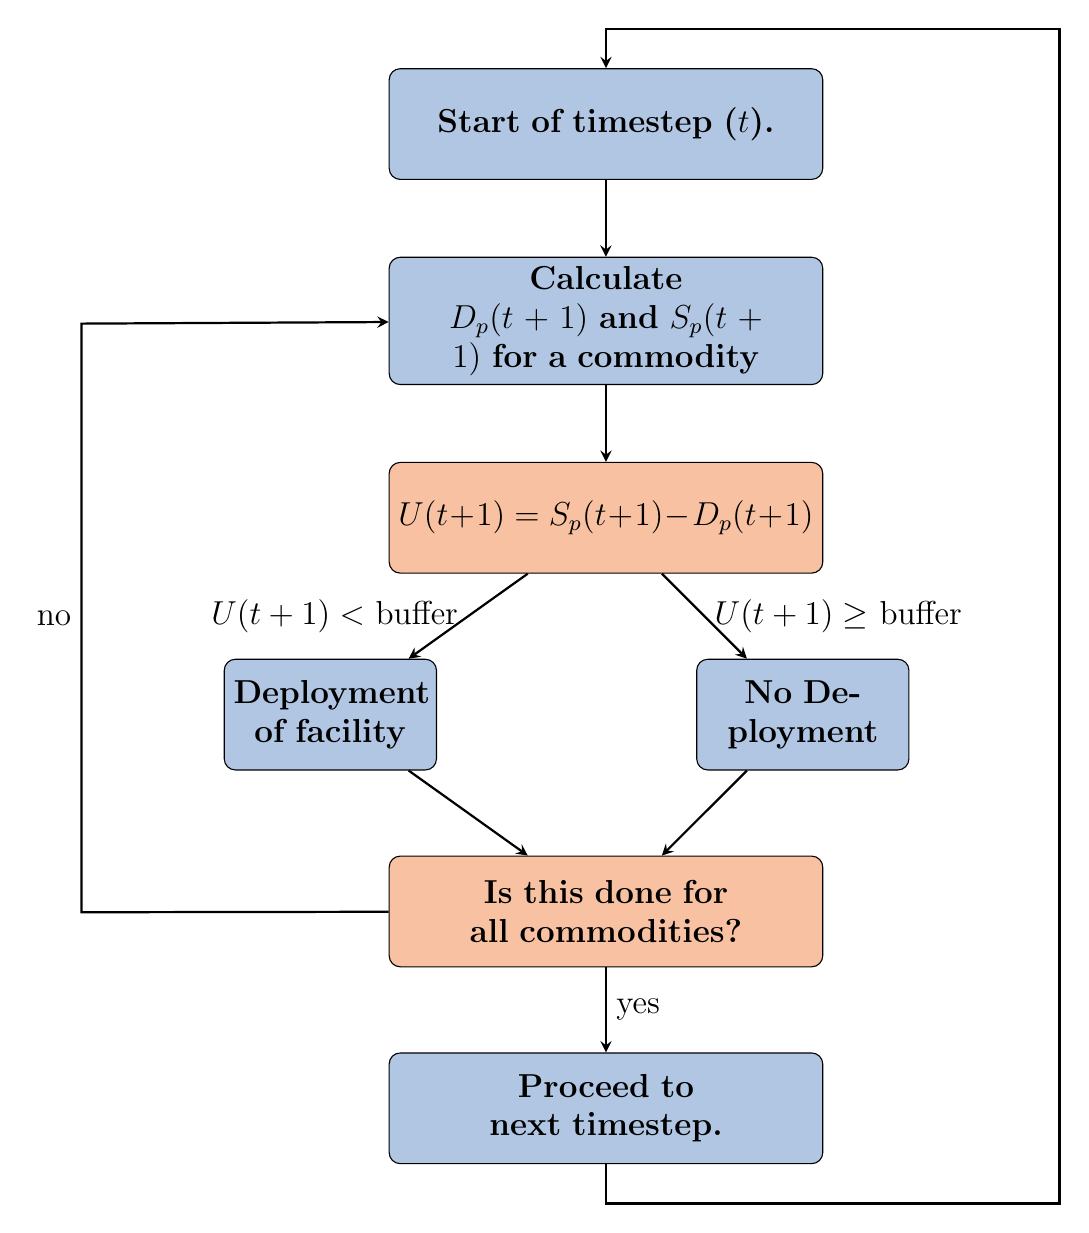
\begin{tikzpicture}[node distance=2.5cm]
        \tikzstyle{every node}=[font=\large]
        \node (Start) [bblock] {\textbf{Start of timestep ($t$).}};
        \node (Predict) [bblock, below of=Start] {\textbf{Calculate \\ $D_p(t+1)$ and $S_p(t+1)$ for a commodity}};
        \node (IsThere) [oblock, below of=Predict]{\textbf{$U(t+1) = S_p(t+1)-D_p(t+1)$}};
        \node (Deploy) [sbblock, below of=IsThere, xshift = -3.5cm]{\textbf{Deployment \\ of facility}};
        \node (NoDeploy) [sbblock, right of=Deploy, xshift = 3.5cm]{\textbf{No Deployment} };
        \node (All) [oblock, below of=Deploy, xshift = 3.5cm] {\textbf{Is this done for all commodities?}};
        \node (End) [bblock, below of=All] {\textbf{Proceed to next timestep.}};
        
        \draw [arrow] (Start) -- (Predict); 
        \draw [arrow] (Predict) -- (IsThere);
        \draw [arrow] (IsThere) -- node[anchor=east] {$U(t+1) <$ buffer} (Deploy);
        \draw [arrow] (IsThere) -- node[anchor=west] {$U(t+1) \geq$ buffer} (NoDeploy);
        \draw [arrow] (Deploy) -- (All);
        \draw [arrow] (NoDeploy) -- (All);
        \draw [arrow] (All) -- node[anchor=west] {yes} (End);
        \draw [arrow] (All) -- ([shift={(-3.9cm,0.7cm)}]All.south west)-- node[anchor=east] {no} ([shift={(-3.9cm,-0.85cm)}]Predict.north west)--(Predict);
        \draw [arrow] (End) |-([shift={(3cm,-0.5cm)}]End.south east)-- ([shift={(3cm,0.5cm)}]Start.north east)-|(Start);
    \end{tikzpicture}
\end{figure}

\deploy's overall objective is to ensure that there is no 
undersupply of power. 
The sub-objectives are : (1) to minimize the number of time 
steps of undersupply or under capacity of any 
commodity, (2): to minimize excessive oversupply of all commodities.
This is a reflection of reality in which it is important to 
never have an undersupply of power on the grid by ensuring power 
plants are never undersupplied of fuel, while not 
having excessive over supply resulting in a burden to store unused 
supplies. 
One of the key issues that \gls{NFCSim}s face is that despite
sufficient installed reactor capacity to meet the power 
demand, there is insufficient supply of fabricated/reprocessed 
fuel at certain timesteps, resulting in idle capacity.  

\subsection{\textbf{Structure}}
%Description of front end and back end of fuel cycle 
%Demand Driven vs. Supply Driven 
In \deploy, two different institutions were implemented for 
front-end and back-end fuel cycle facilities: 
\texttt{DemandDrivenDeploymentInst} and 
\texttt{SupplyDriven} 
\noindent
\texttt{DeploymentInst} respectively. 
This distinction was made because front-end facilities 
are deployed to meet demand for the commodity they produce. 
Whereas, back-end facility are deployed to meet supply for the 
commodity they provide capacity for. 
For example, for front end facilities, a reactor facility 
demands fuel and \texttt{DemandDrivenDeploymentInst} 
triggers deployment of fuel fabrication facilities to create 
supply meeting demand for fuel to prevent undersupply. 
For back end facilities, the reactor generates spent fuel and 
\texttt{SupplyDrivenDeploymentInst} triggers deployment of 
waste storage facilities to create capacity meeting the supply 
of spent fuel to prevent under capacity. 

\subsection{\textbf{Input Variables}}
Table \ref{tab:inputs} lists and gives examples of the input 
variables \deploy accepts. 
Essentially, the user must define the facilities controlled by 
\deploy, their respective capacities, the driving commodity, 
its demand equation, deployment driving method, and prediction method 
for supply and demand. 
The user also has the optional option to define supply/capacity buffers 
for each commodity, facility preferences, and facility constraints. 
In-depth descriptions of the deployment driving method, prediction 
methods, preferences, and buffers are provided in the subsequent sections. 

\begin{table}[]
    \centering
	\resizebox{0.7\textwidth}{!}{%
	\begin{tabular}{|l|l|p{7cm}|}
	\hline
											  & \textbf{Input Parameter}                                                           & \textbf{Examples}                                                                                                          \\ \hline
	\multirow{5}{*}{\textbf{Required}} & Demand driving commodity                                                           & Power, Fuel, Plutonium, etc.                                                                                                                      \\ \cline{2-3} 
											  & Demand equation                                                                    & P(t) = 10000, sin(t), 10000*t                                                                                                                 \\ \cline{2-3} 
											  & Facilities it controls                                                             & Fuel Fab, LWR reactor, SFR reactor, Waste repository, etc.                                                                                                      \\ \cline{2-3} 
											  & Capacities of the facilities                                                       & 3000 kg, 1000 MW, 50000 kg                                                                                                     \\ \cline{2-3} 
											  & Prediction method                                                                  & \begin{tabular}[c]{@{}l@{}}Power: fast fourier transform\\ Fuel: moving average\\ Spent fuel: moving average\end{tabular} \\ \cline{2-3} 
											  & Deployment driven by & Installed Capacity/Supply                                                                                                                    \\ \hline
	\multirow{4}{*}{\textbf{Optional}} & Supply/Capacity Buffer type                                                                        & Absolute                                                                                                                  \\ \cline{2-3} 
											  & Supply/Capacity Buffer size                                                                        & \begin{tabular}[c]{@{}l@{}}Power: 3000 MW\\ Fuel: 0 kg \\ Spent fuel: 0 kg\end{tabular}                                   \\ \cline{2-3} 
											  & Facility preferences                                                               & \begin{tabular}[c]{@{}l@{}}LWR reactor = 100-t\\ SFR reactor = t-100 \end{tabular}          \\ \cline{2-3} 
											  & Facility constraint                                                              & SFR reactor constraint = 5000kg of Pu            \\ \hline	
			
											\end{tabular}%
	}
	\caption{\deploy's required and optional input parameters with examples.}
	\label{tab:inputs}
    \end{table}

    \subsection{\textbf{Deployment Driving Method}}
    The user has the choice of deploying facilities based on the difference 
    between predicted supply and demand, or predicted demand and 
    installed capacity. 
    There are two advantages of using installed capacity over predicted 
    supply. 
    First, to prevent over deployment of facilities that have an
    intermittent supply. 
    For example, reactor facilities have a periodic refueling time. 
    A user might not want \deploy to deploy more reactor facilities 
    to make up for the lack of power supply caused by the gap in 
    supply during refueling. 
    Second, to prevent infinite deployment of a facility that uses 
    a commodity that is no longer available in the simulation. 
    For example, in a transition scenario from \gls{LWR}s to \gls{SFR}s, 
    the reprocessing plant that fabricates \gls{SFR} fuel might demand 
    Pu after the inventory accumulated by \gls{LWR}s is used up 
    and there are no more \gls{LWR} facilities to generate Pu. 
    This will result in \deploy deploying infinite reprocessing 
    facilities to generate \gls{SFR} fuel despite the lack of input Pu 
    to generate it. 
    This can be avoided by using \deploy's facility constraint capability 
    to constrain \gls{SFR} deployment until a sizable inventory of Pu 
    is accumulated in the simulation. 
    
    \subsection{\textbf{Supply/Capacity Buffer}}
    In \texttt{DemandDrivenDeploymentInst}, the user has the option 
    to provide a supply buffer for each commodity so that 
    \deploy will deploy facilities to meet predicted demand and the
    additional buffer value. 
    In \texttt{SupplyDrivenDeploymentInst}, the user has the option 
    to provide a capacity buffer to specific commodities so that 
    \deploy will deploy facilities to meet predicted supply and the
    additional buffer.
    For example, the user could set the power commodity's supply buffer 
    to be 2000 MW. 
    If predicted demand is 10000 MW, \deploy will deploy reactor 
    facilities to meet the predicted demand and supply buffer, resulting 
    in a power supply of 12000 MW.  
    The buffer can be defined as a percentage (equation \ref{eq:perc}) 
    or absolute value (equation \ref{eq:abs}). 
    
    \begin{equation}
        \label{eq:perc}
        S_{pwb} = S_{p}*(1+d)
    \end{equation}
    \begin{equation}
        \label{eq:abs}
        S_{pwb} = S_{p}+a
    \end{equation}
    where $S_{pwb}$ is predicted supply/capacity with buffer, 
    $S_p$ is the predicted supply/capacity without buffer, 
    $d$ is the percentage value in decimal form, 
    and $a$ is the absolute value of the buffer. 
    
    Using a combination of this buffer capability with the 
    installed capacity deployment driving method in a transition 
    scenario simulation is effective in minimizing undersupply of a 
    commodity without having excessive over supply. 
    This is demonstrated in section \ref{sec:demo}. 
    
    \subsection{\textbf{Preferences}}
    % Need to explain the order of preferences for deployment 
    % Constraint, pref, minimize number of facilities and minimize 
    % over supply 
    The user has the option to provide each facility with
    a time dependent preference equation that governs preference for 
    that facility compared to other facilities that provide the same 
    commodity. 
    In the example for facility preferences in table \ref{tab:inputs}, 
    the \gls{LWR} reactor has a preference of $100-t$ and the 
    \gls{SFR} reactor has a preference of $t-100$. 
    Thus, the \gls{LWR} is preferred before time step 100 and \gls{SFR}
    is preferred after. 
    
    The user also has the option to provide each facility with a 
    commodity constraint. 
    In the example for facility constraint in table \ref{tab:inputs}, 
    the \gls{SFR} has a commodity constraint of 5000kg of Pu. 
    This constrains \gls{SFR} deployment by the size of the Pu inventory 
    in the simulation. 
    Once, the 5000kg Pu inventory is first met, \gls{SFR} reactors can 
    henceforth be deployed. 
    
    One of the key issues faced in transition scenarios is the lack 
    of Pu in a scenario that results in idle advanced reactor capacity. 
    Therefore, the facility preferences and constraint capabilities 
    are useful and necessary for modeling transition scenarios. 
    An ideal transition year is selected using the facility 
    preferences, however the transition will only begin when there 
    is sufficient Pu inventory (set by facility constraint) 
    to avoid Pu shortages. 
    
    Therefore, when \deploy predicts an undersupply of a commodity, 
    it deploys available facilities to meet the predicted demand. 
    It will deploy the facility with the highest preference first, 
    unless it does not meet it's constrained criteria, then it will 
    deploy the second most, and so on. 
    If the facilities do not have preferences or constraints, \deploy 
    will deploy the available facilities to minimize the number of 
    deployed facilities while minimizing oversupply of the commodity.

\subsection{\textbf{Prediction Methods}}


\section{Sensitivity Analysis Capabilities}
In this work, \Cyclus and DYMOND are coupled with Dakota 
\cite{eldred_dakota_2010} to give the \glspl{NFCSim} \gls{SA}, 
\gls{UQ}, and optimization capabilities. 
The reason for wrapping \Cyclus and DYMOND with Dakota instead of 
using other sensitivity analysis tools (Python packages etc.)
is because Dakota is a well supported \gls{SA}, \gls{UQ}, 
and optimization tool that provides a flexible interface between 
analysis codes and iterative system analysis methods 
\cite{turner_virtual_nodate}. 
It has also previously been coupled with other nuclear engineering 
softwares \cite{turner_virtual_nodate,zhang_uncertainty_nodate}. 
The parameters for the \gls{SA}, \gls{UQ}, or optimization study is defined 
in the Dakota input file. 

The process of coupling with Dakota are similar 
for both \glspl{NFCSim}. 
The coupling is depicted in Figure \ref{fig:dakota-NFC-flow} in which 
Dakota is applied as a wrapper around each of the \glspl{NFCSim}. 
In this work, a Python interface between Dakota and the \glspl{NFCSim}
are developed. 
The Python interface has three main capabilities: 
(1) it edit the \gls{NFCSim}'s input file with Dakota's input values, 
(2) runs the simulation with the newly edited \gls{NFCSim} input file, and 
(3) reads the \gls{NFCSim}'s output file and returns values of interest 
to the Dakota output file. 
The differences in coupling lies in the python interface to each 
\gls{NFCSim}. 

\begin{figure}[]
    \centering
    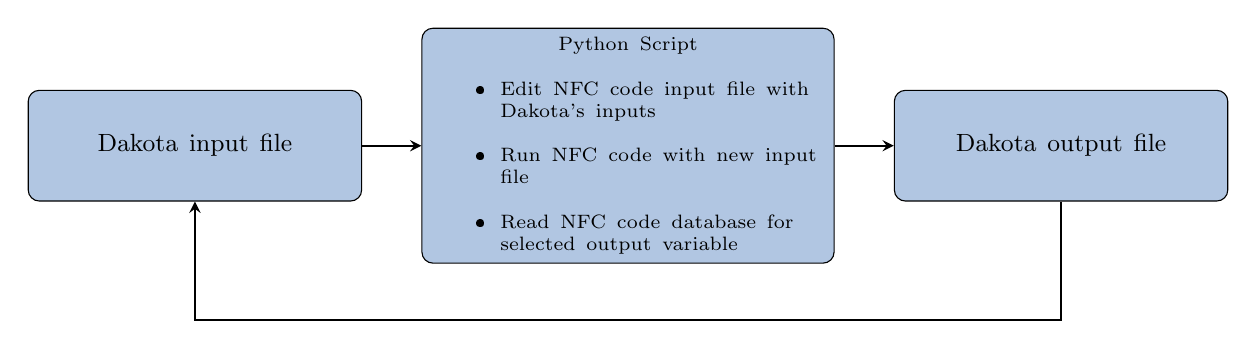
\begin{tikzpicture}[node distance=4.5cm]
        \tikzstyle{every node}=[font=\large]
        \node (one) [sbblock,text width=4cm]{\small Dakota input file};
    \node (two) [bblock, right of=one, xshift = 1cm, text width=5cm]{\scriptsize Python Script\begin{itemize}
        \item Edit NFC code input file with Dakota's inputs 
        \item Run NFC code with new input file 
        \item Read NFC code database for selected output variable
    \end{itemize}};
    \node  (three) [sbblock, xshift = 1cm, right of=two,text width=4cm]{\small Dakota output file};
        
        \draw [arrow] (one) -- (two);
        \draw [arrow] (two) -- (three);
        \draw [arrow] (three) |-([shift={(0cm,-1.5cm)}]three.south west)-- ([shift={(0cm,-1.5cm)}]one.south east)-|(one);
    \end{tikzpicture}
    \caption{Depiction of coupling of Dakota and NFC code}
    \label{fig:dakota-NFC-flow}
\end{figure}

\subsection{Dymond-Dakota Coupling}
% python scripts to parse the excel input and output templates 
In the interface between Dymond and Dakota, Python is used 
to parse the excel input file to edit the relevant 
excel cells accordingly. 
Python is also used to parse the excel output database and take 
values of interest and format them to evaluate the results 
or return to the dakota output file.
The scripts coupling Dymond and Dakota are demonstrated in the 
\texttt{ddwrapper} github repository \cite{ddwrapper_doi_2019}.

\subsection{\Cyclus-Dakota Coupling}
% python scripts + jinja2 for input 
% python scripts + cymetric for output 
In the interface between \Cyclus and Dakota, 
the Jinja2 \cite{ronacher_welcome_2018} package is used 
with Python to edit the relevant parts of \Cyclus' xml input file. 
Jinja2 is a modern and designer-friendly templating 
language for Python. 
The \textsc{Cymetric} \cite{scopatz_cymetric_2015} package is used with Python 
to analyze the \Cyclus output database. 
\textsc{Cymetric} is a general analysis library and tool that was 
created in 2015 to more easily interact with \Cyclus' SQL 
database. 
The scripts coupling \Cyclus and Dakota are demonstrated in the 
\texttt{dcwrapper} github repository \cite{ddwrapper_doi_2019}.


% Add github doi 



\chapter{Successful Transition Scenarios}

\section{Demonstration}
This section will demonstrate and evaluate 
setting up of successful transition scenarios 
with \Cyclus and DYMOND. 
The overall measure of a successful transition scenario  
is that there is no undersupply of power. 
The sub-measures are: 
(1) to minimize the number of time 
steps of undersupply or under capacity of any 
commodity, 
(2) to minimize excessive oversupply of all commodities.

% difference between cyclus and dymond 
% cyclus is more flexible but harder to use 
% dymond is rigid in the type of scenarios to run 
% more comparisons of cyclus and dymond in this section 
%or after demonstration. 
\chapter{Results: Sensitivity Analysis}
In this chapter, DYMOND and \Cyclus are used to conduct 
sensitivity analysis studies of the 
EG01-30 \gls{NFC} transition scenario. 
Dakota-\Cyclus (\texttt{dcwrapper}) 
and Dakota-DYMOND coupling (\texttt{ddwrapper})
perform  
one-at-a-time sensitivity analysis (SA), synergistic 
SA, and global SA. 
This chapter has six sections: 
\begin{enumerate}
    \item Transition Scenario Specifications 
    \item Sensitivity Analysis Evaluation Metrics 
    \item One-at-a-time \gls{SA}
    \item Synergistic \gls{SA}
    \item Global \gls{SA}
    \item Main Takeaways 
\end{enumerate}

\section{Transition Scenario Specification}
% improve this section 
Both DYMOND and \Cyclus sensitivity analyses 
use the EG01-30 transition scenario.
Slight differences lie in the values of some input variables. 

\subsection{DYMOND}
The specifications of the EG01-30 transition scenario used in the 
DYMOND sensitivity analysis
are described in the DYMOND OECD benchmark transition 
scenario presented at the 17th Meeting of Expert Group on Advanced 
Fuel Cycle Scenarios in France in 2017 
\cite{oecd_nuclear_energy_agency_wpfc_nodate}. 
The OECD benchmark scenario is based on the EG01-30 transition scenario 
in which a \gls{PWR} fleet is transitioned to
a mixed fleet of \gls{MOX} \glspl{PWR} and \glspl{SFR}. 
Table \ref{tab:dymondinputs} describe high-level OECD benchmark transition 
scenario specifications. 

\begin{table}[H]
    \centering
    \doublespacing
    \caption{OECD Benchmark Transition Scenario
	Specifications \cite{oecd_nuclear_energy_agency_wpfc_nodate}}
	\label{tab:dymondinputs}
    \small
    \begin{tabular}{ll}
    \hline
                               \textbf{Input Parameter}            & \textbf{Value}            \\ \hline
    Demand driving commodity   & Power              \\
                               Demand equation {[}TWhe/y{]}   & 430        \\
                               Transition Start Date [Year] & 80\\ 
                               Fleet share ratio [\%] & \gls{MOX} \gls{PWR}: 15\%, \gls{SFR}: 85\%\\ \hline
    \end{tabular}%
    \end{table}

\subsection{\Cyclus}
\Cyclus transition scenario sensitivity analysis uses 
the linearly increasing power demand EG01-30 transition scenario 
(described in Section \ref{sec:eg01-30}).  
Figure \ref{fig:30flow} shows the facility and mass flow 
for this transition scenario in \Cyclus. 
Tables \ref{tab:bestinputs} and \ref{tab:facinputs}
shows the input parameters for \deploy and facilities
in the transition scenario. 
The \texttt{reactor} facility used in the \Cyclus simulation 
is a recipe reactor; it accepts a fresh fuel recipe and outputs 
a spent fuel recipe. 
The recipes used for the \gls{LWR}, \gls{MOX} \gls{LWR}, and 
\gls{SFR} are based on recipes generated by VISION 
\cite{chee_arfc/transition-scenarios_2018}
that closely match EG30 scenario specifications in 
Appendix B of the \gls{DOE} Evaluation and Screening Study 
(E\&S study) \cite{wigeland_nuclear_2014}. 

\begin{table}[H]
    \centering
    \doublespacing
    \caption{\Cyclus facility input parameters for
	EG01-EG30 transition scenario
	that minimizes undersupply for power and minimizes 
	the undersupply and under capacity for other facilities. }
	\label{tab:facinputs}
    \small
    \begin{tabular}{lll}
        \hline
        \textbf{Facility}                 & \textbf{Input Parameter}                    & \textbf{Value} \\ \hline
        \multirow{4}{*}{\textbf{LWR}}     & Lifetime {[}months{]}              & 960   \\
                                 & Cycle time {[}months{]}            & 18    \\
                                 & Refuel time {[}months{]}           & 1     \\
                                 & Rated Power {[}MWe{]}              & 1000  \\ \hline
        \multirow{2}{*}{\textbf{MOX LWR}} & Lifetime {[}months{]}              & 960   \\
                                 & Cycle time {[}months{]}            & 18    \\
                                 & Refuel time {[}months{]}           & 1     \\
                                 & Rated Power {[}MWe{]}              & 1000  \\ \hline
        \multirow{4}{*}{\textbf{SFR}}     & Lifetime {[}months{]}              & 720   \\
                                 & Cycle time {[}months{]}            & 12    \\
                                 & Refuel time {[}months{]}           & 1     \\
                                 & Rated Power {[}MWe{]}              & 333   \\ \hline
        \textbf{Cooling Pools}            & Used fuel storage time {[}years{]} & 3  \\ \hline
        \end{tabular}
    \end{table}

\section{Sensitivity Analysis: Evaluation Metrics}
Important optimization metrics and their associated output variables 
must be defined to determine the basis of comparison for sensitivity 
analysis of \gls{NFC} transition scenarios.
The E\&S study \cite{wigeland_nuclear_2014} evaluated transition 
scenarios using nine metrics: nuclear waste 
management, proliferation risk, nuclear material security risk, 
safety, environmental impact, resource utilization, development 
and deployment risk, institutional issues, financial risk, and 
economics. 
These nine metrics can be narrowed down into four categories
 \cite{passerini_systematic_2014}: environmental 
impact, economics, proliferation risk and resource utilization. 

It is necessary to define output indicators to measure the 
impact of the variation of an input parameter on an output 
parameter \cite{noauthor_effects_2017}. 
Output indicators are introduced because the output variables
are a time series resulting in a need for a single value that 
is representative of the output parameter's time series.  
Four types of output indicators are introduced 
\cite{noauthor_effects_2017}: 
(1) final value at the end of simulation
(2) maximum value during simulation,  
(3) cumulative sum over the whole simulation, and 
(4) quality of Plutonium (equation \ref{eq:pu}). 
A different output indicator is used depending on 
the nature of the output parameter.

\begin{align}
    \label{eq:pu}
Quality\ of\ Pu = \frac{Pu_{239}+Pu_{241}}{Pu_{238}+Pu_{240}+Pu_{242}+Pu_{243}+Pu_{244}}
\end{align}

Table \ref{tab:category-output-DD} shows the four evaluation 
metrics and the associated output variables used in this work. 

\begin{table}[H]
    \centering
    \doublespacing
    \caption {Evaluation metrics and their associated output 
    variables for sensitivity analysis.}
	\label{tab:category-output-DD}
        \small
        \begin{tabular}{lll}	
            	\hline
            \textbf{Evaluation Metrics} & \textbf{Output Variable} & \textbf{Indicators}\\
            \hline
            \textbf{Waste Management} & \begin{tabular}[c]{@{}l@{}}Total High Level Waste Inventory\\ Depleted Uranium\end{tabular} & \begin{tabular}[c]{@{}l@{}}Final \\ Final \end{tabular}\\
            \hline
            \textbf{Proliferation Risk} &  \begin{tabular}[c]{@{}l@{}}Pu in Cooling Pools\\ Separated Pu in Storage \\ Separated Pu in HLW \\ 
            \end{tabular} & 
        \begin{tabular}[c]{@{}l@{}} Max, Quality\\ Max, Quality \\ Max, Quality \end{tabular} \\
            
            \hline
            \textbf{Resource Utilization} & Uranium ore consumed & Sum\\
            \hline
            \textbf{Goodness of Transition} & \begin{tabular}[c]{@{}l@{}}Total Idle Capacity\\ Date of Final Idle Capacity \\ Length of transition\end{tabular} & \begin{tabular}[c]{@{}l@{}}Sum \\ Final \\ -\end{tabular} \\ 
            \hline
            \end{tabular}
\end{table}

The operational conditions for the advanced reactors and
the specifics of the transition scenario are variable
since the fuel cycle simulator is modeling future 
trajectories. 
In the transition scenarios, we vary the following 
input parameters: 
\begin{itemize}
    \item Length of used fuel cooling time 
    \item Fleet share ratio of PWR MOX and SFR reactors 
	\item Introduction date of advanced reactor technology
\end{itemize}

In the following sections, 
we conduct one-at-a-time, synergistic, and global
sensitivity analysis of these three input parameters and 
quantify the evaluation metric impact.  

\section{One-at-a-time Sensitivity Analysis}
\label{sec:oat}

\subsection{Length of cooling time for used fuel}
In the DYMOND and \Cyclus EG01-30 transition scenarios, 
we varied used fuel cooling time from 0 to 8 years. 
These simulations are compared based on the evaluation 
metrics described in Table \ref{tab:category-output-DD}.

\subsubsection{\textbf{DYMOND}}
Tables \ref{tab:dymond-ct-1} and \ref{tab:dymond-ct-2} show 
the absolute values of 
output variables associated with the environmental impact, 
resource utilization, and goodness of transition evaluation 
metrics for each scenario. 
Tables \ref{tab:dymond-ct-sa-1} and \ref{tab:dymond-ct-sa-2} 
show each scenario's percentage 
difference compared with the base case of `Cooling Time = 2 years'
scenario.

In Table \ref{tab:dymond-ct-1}, total idle capacity 
in the simulation increases for used fuel cooling time of 3 years 
onwards. 
This is because the fuel management strategy in the 
DYMOND OECD benchmark scenario was 
manually edited to work best with a 2 year used fuel cooling time.
The idle capacity in cooling time of 3 years onwards could be 
avoided by manually changing the fuel management strategy
in the DYMOND input file for the scenario. 
We did not manually change the fuel management strategy
because this is a one-at-a-time \gls{SA} study 
and, thus, only used fuel cooling time was varied. 

In Table \ref{tab:dymond-ct-sa-2}, compared to the base case, 
as cooling time increases, maximum Pu in the cooling pools increases.
This is expected since there is a larger inventory of used fuel 
in the cooling pools when cooling time increases. 
The quality of Pu in the cooling pools also increases as cooling time 
increases. 
% add more description?  

\begin{table}[H]
    \centering
    \caption{DYMOND: Assessment of how variation of used fuel cooling times
    impacts evaluation metrics (waste management, resource utilization, 
    and goodness of transition) for OECD benchmark transition scenario.}
	\label{tab:dymond-ct-1}
        \scriptsize
        \begin{tabularx}{\textwidth}{R|RR|R|RRR}	
            \hline
            \textbf{} & \multicolumn{2}{c|}{\textbf{Environmental Impact}}                                                                                                                                                                                                                                                      & \textbf{Resource Utilization}                                                                                        & \multicolumn{3}{c}{\textbf{Goodness of Transition}}                                                                                                                                                                                 \\ \hline
\textbf{Scenario: Used Fuel Cooling Time [Year]} & \textbf{Final HLW [kg] } & \textbf{Final Depleted U [kg]} &  \textbf{Total Mined Uranium Ore [kg]}  & \textbf{Total Idle Capacity[kg]} & \textbf{Year of Final Idle Capacity} & \textbf{Length of Transition [years]} \\ \hline
 0  &           1103.2 &                             916933.4 &                       16188.8 &                                    30148.8 &                      301 &                     227 \\ 
 1  &           1101.6 &                             916618.2 &                       16188.8 &                                    30148.8 &                      301 &                     227 \\ 
 2  &           1105.7 &                             916237.60 &                       16188.8 &                                    30148.8 &                      301 &                     227 \\ 
 3  &           1108.3 &                             916268.7 &                       16188.8 &                                   256588.8 &                      301 &                     227 \\ 
 4  &           1099.8 &                             916962.4 &                       16188.8 &                                 1338604.8 &                      301 &                     227 \\ \hline
\end{tabularx}%
\end{table}

\begin{table}[H]
    \centering
    \caption{DYMOND: Assessment of how variation of used fuel cooling times
    impacts evaluation metrics (proliferation risk) for OECD benchmark
	transition scenario.}
	\label{tab:dymond-ct-2}
        \scriptsize
        \begin{tabularx}{\textwidth}{R|RRRRRR}	
            \hline
            \textbf{} & \multicolumn{6}{c}{\textbf{Proliferation Risk}}  \\ \hline
\textbf{Scenario: Used Fuel Cooling Time [Year]} & \textbf{Max Pu in cooling pools [kg] } & \textbf{Pu Quality at max Pu in cooling pools [kg]} &  \textbf{Max Pu in HLW [kg]}  & \textbf{Pu Quality at max Pu in HLW [kg]} & \textbf{Max Pu in Rpr facilities [kg]} & \textbf{Pu Quality at max Pu in Rpr facilities [kg]} \\ \hline
 0  &           0.0 &                             0 &                       18.374 &                                    0.650 &                      208.6 &                     - \\ 
 1  &           105.2 &                             0.652 &                       18.385 &                                    0.652 &                      208.6 &                     - \\ 
 2  &           196.8 &                             0.622 &                       18.409 &                                    0.653 &                      208.6 &                     - \\ 
 3  &           264.8 &                             0.659 &                       18.189 &                                   0.654 &                      208.6 &                     - \\ 
 4  &           348.2 &                             0.671 &                       16.805 &                                 0.658 &                      208.6 &                     - \\ \hline
\end{tabularx}%
\end{table}

\begin{table}[H]
    \caption{DYMOND: Sensitivity analysis of how variation of used fuel 
    cooling times impacts evaluation metrics (waste management, resource utilization, 
    and goodness of transition) for OECD benchmark transition scenario.
    The numbers in the table represent the percentage difference between 
    an output variable from each scenario and the base case scenario (Cooling time = 2 years).}
    \label{tab:dymond-ct-sa-1}
    \scriptsize
    \begin{tabularx}{\textwidth}{R|RR|R|RRR}	
		\hline
        \textbf{} & \multicolumn{2}{c|}{\textbf{Environmental Impact}}                                    & \textbf{Resource Utilization}                                                                                       & \multicolumn{3}{c}{\textbf{Goodness of Transition}}                                                                                                                                                                                 \\ \hline
        \textbf{Scenario: Used Fuel Cooling Time [Year]} & \textbf{Final HLW [\%] } & \textbf{Final Depleted U [\%]} &  \textbf{Total Mined Uranium Ore [\%]]}  & \textbf{Total Idle Capacity [\%]} & \textbf{Year of Final Idle Capacity [\%]} & \textbf{Length of Transition [\%]} \\ \hline
         0  &             \cellcolor[HTML]{67FD9A}-0.221736 &                                   \cellcolor[HTML]{67FD9A}0.075939 &                                                            \cellcolor[HTML]{67FD9A}0.0 &                 \cellcolor[HTML]{67FD9A}0.000000 &                                           \cellcolor[HTML]{67FD9A}0.0 & \cellcolor[HTML]{67FD9A}0.0 \\
		 1  &             \cellcolor[HTML]{67FD9A}-0.363540 &                                    \cellcolor[HTML]{67FD9A}0.041532 &                                                           \cellcolor[HTML]{67FD9A}0.0 &                 \cellcolor[HTML]{67FD9A}0.000000 &                                          \cellcolor[HTML]{67FD9A}0.0 & \cellcolor[HTML]{67FD9A}0.0 \\ 
		 2  &              \cellcolor[HTML]{000000}0.000000 &                                     \cellcolor[HTML]{000000}0.000000 &                                                              \cellcolor[HTML]{000000}0.0 &                 \cellcolor[HTML]{000000}0.000000 &                                         \cellcolor[HTML]{000000}0.0 & \cellcolor[HTML]{000000}0.0 \\ 
		 3  &              \cellcolor[HTML]{67FD9A}0.234524 &                                    \cellcolor[HTML]{67FD9A}0.003389 &                                                              \cellcolor[HTML]{67FD9A}0.0 &               \cellcolor[HTML]{FD6864}751.074670 &                                         \cellcolor[HTML]{67FD9A}0.0 & \cellcolor[HTML]{67FD9A}0.0 \\ 
		 4  &             \cellcolor[HTML]{67FD9A}-0.529033 &                                   \cellcolor[HTML]{67FD9A}0.079102 &                                                        \cellcolor[HTML]{67FD9A}0.0 &              \cellcolor[HTML]{FD6864}4339.993632 &                                        \cellcolor[HTML]{67FD9A}0.0 & \cellcolor[HTML]{67FD9A}0.0 \\ \hline
	\end{tabularx}%
    
    \resizebox{0.3\textwidth}{!}{
    \fbox{\begin{tabular}{ll}
        \textcolor{green}{$\blacksquare$} & $sensitivity \leq 1\%$ \\
        \textcolor{orange}{$\blacksquare$} & $1\% < sensitivity < 10\%$ \\
        \textcolor{red}{$\blacksquare$} & $sensitivity \geq 10\%$
        \end{tabular}}}
    \end{table}

    \begin{table}[H]
        \caption{DYMOND: Sensitivity analysis of how variation of used fuel 
        cooling times impacts evaluation metrics (proliferation risk)for OECD benchmark transition scenario.
        The numbers in the table represent the percentage difference between 
    an output variable from each scenario and the base case scenario (Cooling time = 2 years).}
        \label{tab:dymond-ct-sa-2}
        \scriptsize
        \begin{tabularx}{\textwidth}{R|RRRRRR}	
            \hline
            \textbf{} & \multicolumn{6}{c}{\textbf{Proliferation Risk}}  \\ \hline
\textbf{Scenario: Used Fuel Cooling Time [Year]} & \textbf{Max Pu in cooling pools [\%] } & \textbf{Pu Quality at max Pu in cooling pools [\%]} &  \textbf{Max Pu in HLW [\%]}  & \textbf{Pu Quality at max Pu in HLW [\%]} & \textbf{Max Pu in Rpr facilities [\%]} & \textbf{Pu Quality at max Pu in Rpr facilities [\%]} \\ \hline
             0  &             \cellcolor[HTML]{FD6864}-100 &                                   \cellcolor[HTML]{FD6864}-100 &                                                            \cellcolor[HTML]{67FD9A}-0.19 &                 \cellcolor[HTML]{67FD9A}-0.459 &                                           \cellcolor[HTML]{67FD9A}0.0 & \cellcolor[HTML]{67FD9A}- \\
             1  &             \cellcolor[HTML]{FD6864}-46.5 &                                    \cellcolor[HTML]{FE996B}4.82 &                                                           \cellcolor[HTML]{67FD9A}-0.13 &                 \cellcolor[HTML]{67FD9A}-0.153 &                                          \cellcolor[HTML]{67FD9A}0.0 & \cellcolor[HTML]{67FD9A}- \\ 
             2  &              \cellcolor[HTML]{000000}0.000000 &                                     \cellcolor[HTML]{000000}0.000000 &                                                              \cellcolor[HTML]{000000}0.0 &                 \cellcolor[HTML]{000000}0.000000 &                                         \cellcolor[HTML]{000000}0.0 & \cellcolor[HTML]{000000}0.0 \\ 
             3  &              \cellcolor[HTML]{FD6864}34.5 &                                    \cellcolor[HTML]{FE996B}5.95 &                                                              \cellcolor[HTML]{FE996B}-1.20 &               \cellcolor[HTML]{FD6864}0.153 &                                         \cellcolor[HTML]{67FD9A}0.0 & \cellcolor[HTML]{67FD9A}- \\ 
             4  &             \cellcolor[HTML]{FD6864}76.9 &                                   \cellcolor[HTML]{FE996B}7.88 &                                                        \cellcolor[HTML]{FE996B}-8.71 &              \cellcolor[HTML]{FD6864}0.766 &                                        \cellcolor[HTML]{67FD9A}0.0 & \cellcolor[HTML]{67FD9A}- \\ \hline
        \end{tabularx}%
        
        \resizebox{0.3\textwidth}{!}{
        \fbox{\begin{tabular}{ll}
            \textcolor{green}{$\blacksquare$} & $sensitivity \leq 1\%$ \\
            \textcolor{orange}{$\blacksquare$} & $1\% < sensitivity < 10\%$ \\
            \textcolor{red}{$\blacksquare$} & $sensitivity \geq 10\%$
            \end{tabular}}}
        \end{table}

    
\subsubsection{\textbf{\Cyclus}}

Tables \ref{tab:cyclus-ct-1} and \ref{tab:cyclus-ct-2} show 
the absolute values of 
output variables associated with the environmental impact, 
resource utilization, and goodness of transition evaluation 
metrics for each scenario. 
Tables \ref{tab:cyclus-ct-sa-1} and \ref{tab:cyclus-ct-sa-2} 
show each scenario's percentage 
difference compared with the base case of `Cooling Time = 2 years'
scenario.

In Table \ref{tab:cyclus-ct-sa-1}, most evaluation metrics do not change 
for variation in the used fuel cooling time, with exception of the final 
HLW amount in the scenario. 
Final HLW amount decreases for a longer used fuel cooling time.
In Table \ref{tab:cyclus-ct-sa-2}, compared to the base case, 
as cooling time increases, maximum Pu in the cooling pools increases.
This is similar to the result for the DYMOND transition scenario (table 
\ref{tab:dymond-ct-sa-2}). 
This is expected since there will be a larger inventory of used fuel 
in the cooling pools when cooling time increases. 
The quality of Pu in the cooling pools decreases as cooling time 
increases. 
Maximum Pu in HLW and reprocessing facilities, and their corresponding 
Pu quality, decrease for a longer cooling time. 

\begin{table}[H]
    \centering
    \caption{\Cyclus: Assessment of how variation of used fuel cooling times
    impacts evaluation metrics (waste management, resource utilization, 
    and goodness of transition) for OECD benchmark transition scenario.}
	\label{tab:cyclus-ct-1}
        \scriptsize
        \begin{tabularx}{\textwidth}{R|RR|R|RRR}
            \hline	
            \textbf{} & \multicolumn{2}{c|}{\textbf{Environmental Impact}}                                                                                                                                                                                                                                                      & \textbf{Resource Utilization}                                                                                        & \multicolumn{3}{c}{\textbf{Goodness of Transition}}                                                                                                                                                                                 \\ \hline
\textbf{Scenario: Used Fuel Cooling Time [Year]} & \textbf{Final HLW [kg] } & \textbf{Final Depleted U [kg]} &  \textbf{Total Mined Uranium Ore [kg]}  & \textbf{Total Idle Capacity[kg]} & \textbf{Year of Final Idle Capacity} & \textbf{Length of Transition [years]} \\ \hline

0  & 13223828.1 & 798818620.4      & 1.437e11    & 135.1               & 962                     & 2                      \\
2  & 13073261.2 & 798818620.4      & 1.437e11    & 135.1               & 962                     & 2                      \\
4  & 12906058.3 & 798818620.4      & 1.437e11    & 135.1               & 962                     & 2                      \\
6  & 12795682.5 & 798818620.4      & 1.437e11    & 135.1               & 962                     & 2                      \\
8  & 12726528.6 & 798818620.4      & 1.437e11    & 135.1               & 962                     & 2                     \\ \hline 
        \end{tabularx}
\end{table}

\begin{table}[H]
    \centering
    \caption{\Cyclus: Assessment of how variation of used fuel cooling times
    impacts evaluation metrics (proliferation risk) for OECD benchmark
	transition scenario.}
	\label{tab:cyclus-ct-2}
        \scriptsize
        \begin{tabularx}{\textwidth}{R|RRRRRR}	
            \hline
            \textbf{} & \multicolumn{6}{c}{\textbf{Proliferation Risk}}  \\ \hline
\textbf{Scenario: Used Fuel Cooling Time [Year]} & \textbf{Max Pu in cooling pools [kg] } & \textbf{Pu Quality at max Pu in cooling pools [kg]} &  \textbf{Max Pu in HLW [kg]}  & \textbf{Pu Quality at max Pu in HLW [kg]} & \textbf{Max Pu in Rpr facilities [kg]} & \textbf{Pu Quality at max Pu in Rpr facilities [kg]} \\ \hline
0  & 48979.28         & 0.66                           & 44426.65      & 0.62                        & 2800580.69        & 0.49                            \\
2  & 199036.06        & 0.6                            & 43629.18      & 0.62                        & 2637125.07        & 0.48                            \\
4  & 368405.04        & 0.58                           & 42844.4       & 0.62                        & 2460403.99        & 0.48                            \\
6  & 554321.66        & 0.57                           & 42646.72      & 0.62                        & 2290857.92        & 0.47                            \\
8  & 733483.85        & 0.56                           & 42858.1       & 0.62                        & 2111786.28        & 0.47                           \\ \hline
\end{tabularx}%
\end{table}

% add color 
\begin{table}[H]
    \caption{\Cyclus: Sensitivity analysis of how variation of used fuel 
    cooling times impacts evaluation metrics (environmental impact, resource
    utilization, and goodness of transition) for OECD benchmark 
    transition scenario.
    The numbers in the table represent the percentage difference between 
    an output variable from each scenario and the base case scenario (Cooling time = 2 years).}
    \label{tab:cyclus-ct-sa-1}
    \scriptsize
    \begin{tabularx}{\textwidth}{R|RR|R|RRR}	
		\hline
        \textbf{} & \multicolumn{2}{c|}{\textbf{Environmental Impact}}                                    & \textbf{Resource Utilization}                                                                                       & \multicolumn{3}{c}{\textbf{Goodness of Transition}}                                                                                                                                                                                 \\ \hline
        \textbf{Scenario: Used Fuel Cooling Time [Year]} & \textbf{Final HLW [\%] } & \textbf{Final Depleted U [\%]} &  \textbf{Total Mined Uranium Ore [\%]]}  & \textbf{Total Idle Capacity [\%]} & \textbf{Year of Final Idle Capacity [\%]} & \textbf{Length of Transition [\%]} \\ \hline0  & \cellcolor[HTML]{FE996B}1.15      & \cellcolor[HTML]{67FD9A}0.0              & \cellcolor[HTML]{67FD9A}0.0               & \cellcolor[HTML]{67FD9A}0.0                 & \cellcolor[HTML]{67FD9A}0.0                     & \cellcolor[HTML]{67FD9A}0.0                    \\
        2  & \cellcolor[HTML]{000000}0.0       & \cellcolor[HTML]{000000}0.0              & \cellcolor[HTML]{000000}0.0               & \cellcolor[HTML]{000000}0.0                 & \cellcolor[HTML]{000000}0.0                     & \cellcolor[HTML]{000000}0.0                    \\
        4  & \cellcolor[HTML]{FE996B}-1.28       & \cellcolor[HTML]{67FD9A}0.0              & \cellcolor[HTML]{67FD9A}0.0               & \cellcolor[HTML]{67FD9A}0.0                 & \cellcolor[HTML]{67FD9A}0.0                     & \cellcolor[HTML]{67FD9A}0.0                    \\
        6  & \cellcolor[HTML]{FE996B}-2.12     & \cellcolor[HTML]{67FD9A}0.0              & \cellcolor[HTML]{67FD9A}0.0               & \cellcolor[HTML]{67FD9A}0.0                 & \cellcolor[HTML]{67FD9A}0.0                     & \cellcolor[HTML]{67FD9A}0.0                    \\
        8  & \cellcolor[HTML]{FE996B}-2.65     & \cellcolor[HTML]{67FD9A}0.0              & \cellcolor[HTML]{67FD9A}0.0               & \cellcolor[HTML]{67FD9A}0.0                 & \cellcolor[HTML]{67FD9A}0.0                     & \cellcolor[HTML]{67FD9A}0.0                   \\ \hline 
                \end{tabularx}%
    
    \resizebox{0.3\textwidth}{!}{
    \fbox{\begin{tabular}{ll}
        \textcolor{green}{$\blacksquare$} & $sensitivity \leq 1\%$ \\
        \textcolor{orange}{$\blacksquare$} & $1\% < sensitivity < 10\%$ \\
        \textcolor{red}{$\blacksquare$} & $sensitivity \geq 10\%$
        \end{tabular}}}
    \end{table}

    \begin{table}[H]
        \caption{\Cyclus: Sensitivity analysis of how variation of used fuel 
        cooling times impacts evaluation metrics (proliferation risk) for OECD benchmark transition scenario.
        The numbers in the table represent the percentage difference between 
        an output variable from each scenario and the base case scenario (Cooling time = 2 years).}
        \label{tab:cyclus-ct-sa-2}
        \scriptsize
        \begin{tabularx}{\textwidth}{R|RRRRRR}	
            \hline
            \textbf{} & \multicolumn{6}{c}{\textbf{Proliferation Risk}}  \\ \hline
            \textbf{Scenario: Used Fuel Cooling Time [Year]} & \textbf{Max Pu in cooling pools [\%] } & \textbf{Pu Quality at max Pu in cooling pools [\%]} &  \textbf{Max Pu in HLW [\%]}  & \textbf{Pu Quality at max Pu in HLW [\%]} & \textbf{Max Pu in Rpr facilities [\%]} & \textbf{Pu Quality at max Pu in Rpr facilities [\%]} \\ \hline
            0  & \cellcolor[HTML]{FD6864}-75.39           & \cellcolor[HTML]{FE996B}8.99                           & \cellcolor[HTML]{FE996B}1.83          & \cellcolor[HTML]{67FD9A}0.08                        & \cellcolor[HTML]{FE996B}6.2               & \cellcolor[HTML]{FE996B}1.45                            \\
2  &\cellcolor[HTML]{000000}0.0              & \cellcolor[HTML]{000000}0.0                            & \cellcolor[HTML]{000000}0.0           & \cellcolor[HTML]{000000}0.0                         & \cellcolor[HTML]{000000}0.0               & \cellcolor[HTML]{000000}0.0                             \\
4  & \cellcolor[HTML]{FD6864}85.09            & \cellcolor[HTML]{FE996B}-3.34                          & \cellcolor[HTML]{FE996B}-1.8          & \cellcolor[HTML]{67FD9A}-0.12                       & \cellcolor[HTML]{FE996B}-6.7              & \cellcolor[HTML]{FE996B}-1.06                           \\
6  & \cellcolor[HTML]{FD6864}178.5            & \cellcolor[HTML]{FE996B}-5.55                          & \cellcolor[HTML]{FE996B}-2.25         & \cellcolor[HTML]{67FD9A}-0.15                       & \cellcolor[HTML]{FD6864}-13.13            & \cellcolor[HTML]{FE996B}-2.11                           \\
8  & \cellcolor[HTML]{FD6864}268.52           & \cellcolor[HTML]{FE996B}-7.23                          & \cellcolor[HTML]{FE996B}-1.77         & \cellcolor[HTML]{67FD9A}-0.22                       & \cellcolor[HTML]{FD6864}-19.92            & \cellcolor[HTML]{FE996B}-3.0                           \\ \hline
        \end{tabularx}
        \end{table}

\subsection{Fleet share ratio of PWR MOX and SFR reactors}

The fleet share ratio of \gls{MOX} \glspl{PWR} and \glspl{SFR}
was varied from 0\% to 20\% of \gls{MOX} \glspl{PWR} for the 
\Cyclus EG01-30 transition scenario. 
These simulations are compared based on the evaluation 
metrics described in Table \ref{tab:category-output-DD}. 

Tables \ref{tab:cyclus-fs-1} and \ref{tab:cyclus-fs-2} show 
the absolute values of 
output variables associated with the environmental impact, 
resource utilization, and goodness of transition evaluation 
metrics for each scenario. 
Tables \ref{tab:cyclus-fs-sa-1} and \ref{tab:cyclus-fs-sa-2} 
show each scenario's percentage 
difference compared with the base case of `Fleet share = 15\% 
\gls{MOX} \glspl{PWR}' scenario. 

In Table \ref{tab:cyclus-fs-sa-1}, most evaluation metrics do not change 
for variation in fleet share ratio, except for the final 
amount of HLW in the scenario. 
The final amount of HLW is largest for 0\% fleet share of \gls{MOX} 
\glspl{PWR} and decreases as the fleet share of \gls{MOX} \glspl{PWR} 
increases. 
In Table \ref{tab:cyclus-fs-sa-2}, maximum Pu in cooling pools and 
reprocessing facility 
decreases for increasing fleet share ratio of \gls{MOX} \glspl{PWR}; 
however, the quality of Pu increases. 
Maximum Pu in HLW increases for a decreasing fleet share ratio
of \gls{MOX} \glspl{PWR}, while the quality of Pu decreases slightly.
Therefore, if minimizing proliferation risk is a high priority, 
a transition scenario 
with a smaller fleet share of \gls{MOX} \glspl{PWR} is recommended
to minimize the Pu amount in the cooling pools and reprocessing facilities. 

% correct stuff 
\begin{table}[H]
    \centering
    \caption{\Cyclus: Assessment of how variation of fleet share ratio
    of PWR MOX and SFR reactors
    impacts evaluation metrics (environmental impact, resource
    utilization, and goodness of transition) for EG01-30 transition scenario.}
	\label{tab:cyclus-fs-1}
        \scriptsize
        \begin{tabularx}{\textwidth}{R|RR|R|RRR}
            \hline	
            \textbf{} & \multicolumn{2}{c|}{\textbf{Environmental Impact}}                                                                                                                                                                                                                                                      & \textbf{Resource Utilization}                                                                                        & \multicolumn{3}{c}{\textbf{Goodness of Transition}}                                                                                                                                                                                 \\ \hline
\textbf{Scenario: PWR MOX Fleet Share [\%]} & \textbf{Final HLW [kg] } & \textbf{Final Depleted U [kg]} &  \textbf{Total Mined Uranium Ore [kg]}  & \textbf{Total Idle Capacity[kg]} & \textbf{Year of Final Idle Capacity} & \textbf{Length of Transition [years]} \\ \hline

0  & 13153061.6 & 798818620.4      & 1.437e11    & 135.1               & 962                     & 2                      \\
5  & 13056988.7 & 798818620.4      & 1.437e11    & 135.1               & 962                     & 2                      \\
10 & 13051896.3 & 798818620.4      & 1.437e11    & 135.1               & 962                     & 2                      \\
15 & 12959554.1 & 798818620.4      & 1.437e11    & 135.1               & 962                     & 2                      \\
20 & 13002120.9 & 798818620.4      & 1.437e11    & 135.1               & 962                     & 2                     \\ \hline
        \end{tabularx}
\end{table}

% correct stuff 
\begin{table}[H]
    \centering
    \caption{\Cyclus: Assessment of how variation of fleet share ratio
    of PWR MOX and SFR reactors
    impacts evaluation metrics (proliferation risk) for EG01-30 transition scenario.}
	\label{tab:cyclus-fs-2}
        \scriptsize
        \begin{tabularx}{\textwidth}{R|RRRRRR}	
            \hline
            \textbf{} & \multicolumn{6}{c}{\textbf{Proliferation Risk}}  \\ \hline
\textbf{Scenario: PWR MOX Fleet Share [\%]} & \textbf{Max Pu in cooling pools [kg] } & \textbf{Pu Quality at max Pu in cooling pools [kg]} &  \textbf{Max Pu in HLW [kg]}  & \textbf{Pu Quality at max Pu in HLW [kg]} & \textbf{Max Pu in Rpr facilities [kg]} & \textbf{Pu Quality at max Pu in Rpr facilities [kg]} \\ \hline
0  & 256794.03        & 0.66                           & 45816.02      & 0.62                        & 2357604.01        & 0.55                            \\
5  & 273733.13        & 0.62                           & 44338.72      & 0.62                        & 2461421.31        & 0.51                            \\
10 & 279694.78        & 0.61                           & 44055.54      & 0.62                        & 2513133.76        & 0.5                             \\
15 & 285794.85        & 0.59                           & 42905.59      & 0.62                        & 2552142.82        & 0.48                            \\
20 & 291786.54        & 0.58                           & 43133.61      & 0.62                        & 2605589.02        & 0.47                           \\ \hline
\end{tabularx}%
\end{table}

% correct stuff 
\begin{table}[H]
    \caption{\Cyclus: Sensitivity analysis of how variation of fleet share 
    ratio impacts evaluation metrics (environmental impact, resource
    utilization, and goodness of transition) for OECD benchmark 
    transition scenario.
    The numbers in the table represent the percentage difference between 
    an output variable from each scenario and the base case scenario 
    (PWR MOX fleet share = 15\%).}
    \label{tab:cyclus-fs-sa-1}
    \scriptsize
    \begin{tabularx}{\textwidth}{R|RR|R|RRR}	
		\hline
        \textbf{} & \multicolumn{2}{c|}{\textbf{Environmental Impact}}                                    & \textbf{Resource Utilization}                                                                                       & \multicolumn{3}{c}{\textbf{Goodness of Transition}}                                                                                                                                                                                 \\ \hline
        \textbf{Scenario: PWR MOX Fleet Share [\%]} & \textbf{Final HLW [\%] } & \textbf{Final Depleted U [\%]} &  \textbf{Total Mined Uranium Ore [\%]]}  & \textbf{Total Idle Capacity [\%]} & \textbf{Year of Final Idle Capacity [\%]} & \textbf{Length of Transition [\%]} \\ \hline
        0  & \cellcolor[HTML]{FE996B}1.49      & \cellcolor[HTML]{67FD9A}0.0              & \cellcolor[HTML]{67FD9A}0.0               & \cellcolor[HTML]{67FD9A}0.0                 & \cellcolor[HTML]{67FD9A}0.0                     & \cellcolor[HTML]{67FD9A}0.0                    \\
        5  & \cellcolor[HTML]{67FD9A}0.75      & \cellcolor[HTML]{67FD9A}0.0              & \cellcolor[HTML]{67FD9A}0.0               & \cellcolor[HTML]{67FD9A}0.0                 & \cellcolor[HTML]{67FD9A}0.0                     & \cellcolor[HTML]{67FD9A}0.0                    \\
        10 & \cellcolor[HTML]{67FD9A}0.71      & \cellcolor[HTML]{67FD9A}0.0              & \cellcolor[HTML]{67FD9A}0.0               & \cellcolor[HTML]{67FD9A}0.0                 & \cellcolor[HTML]{67FD9A}0.0                     & \cellcolor[HTML]{67FD9A}0.0                    \\
        15 & \cellcolor[HTML]{000000}0.0       & \cellcolor[HTML]{000000}0.0              & \cellcolor[HTML]{000000}0.0               & \cellcolor[HTML]{000000}0.0                 & \cellcolor[HTML]{000000}0.0                     & \cellcolor[HTML]{000000}0.0                    \\
        20 & \cellcolor[HTML]{67FD9A}0.33      & \cellcolor[HTML]{67FD9A}0.0              & \cellcolor[HTML]{67FD9A}0.0               & \cellcolor[HTML]{67FD9A}0.0                 & \cellcolor[HTML]{67FD9A}0.0                     & \cellcolor[HTML]{67FD9A}0.0                   \\ \hline
                       \end{tabularx}%
    
    \resizebox{0.3\textwidth}{!}{
    \fbox{\begin{tabular}{ll}
        \textcolor{green}{$\blacksquare$} & $sensitivity \leq 1\%$ \\
        \textcolor{orange}{$\blacksquare$} & $1\% < sensitivity < 10\%$ \\
        \textcolor{red}{$\blacksquare$} & $sensitivity \geq 10\%$
        \end{tabular}}}
    \end{table}

    % correct stuff 
\begin{table}[H]
    \caption{\Cyclus: Sensitivity analysis of how variation of fleet share 
    ratio impacts evaluation metrics (proliferation risk) for OECD benchmark 
    transition scenario.
    The numbers in the table represent the percentage difference between 
    an output variable from each scenario and the base case scenario
    (PWR MOX fleet share = 15\%).}
    \label{tab:cyclus-fs-sa-2}
    \scriptsize
    \begin{tabularx}{\textwidth}{R|RRRRRR}	
		\hline
        \textbf{} & \multicolumn{6}{c}{\textbf{Proliferation Risk}}  \\ \hline
        \textbf{Scenario: PWR MOX Fleet Share [\%]} & \textbf{Max Pu in cooling pools [\%] } & \textbf{Pu Quality at max Pu in cooling pools [\%]} &  \textbf{Max Pu in HLW [\%]}  & \textbf{Pu Quality at max Pu in HLW [\%]} & \textbf{Max Pu in Rpr facilities [\%]} & \textbf{Pu Quality at max Pu in Rpr facilities [\%]} \\ \hline
0  & \cellcolor[HTML]{FD6864}-10.15           & \cellcolor[HTML]{FD6864}10.63                          & \cellcolor[HTML]{FE996B}6.78          & \cellcolor[HTML]{67FD9A}-0.48                       & \cellcolor[HTML]{FE996B}-7.62             & \cellcolor[HTML]{FD6864}14.05                           \\
        5  & \cellcolor[HTML]{FE996B}-4.22            & \cellcolor[HTML]{FE996B}4.34                           & \cellcolor[HTML]{FE996B}3.34          & \cellcolor[HTML]{67FD9A}-0.21                       & \cellcolor[HTML]{FE996B}-3.55             & \cellcolor[HTML]{FE996B}6.57                            \\
        10 & \cellcolor[HTML]{FE996B}-2.13            & \cellcolor[HTML]{FE996B}2.15                           & \cellcolor[HTML]{FE996B}2.68          & \cellcolor[HTML]{67FD9A}-0.09                       & \cellcolor[HTML]{FE996B}-1.53             & \cellcolor[HTML]{FE996B}3.35                            \\
        15 & \cellcolor[HTML]{000000}0.0              & \cellcolor[HTML]{000000}0.0                            & \cellcolor[HTML]{000000}0.0           & \cellcolor[HTML]{000000}0.0                         & \cellcolor[HTML]{000000}0.0               & \cellcolor[HTML]{000000}0.0                             \\
        20 & \cellcolor[HTML]{FE996B}2.1              & \cellcolor[HTML]{FE996B}-2.02                          & \cellcolor[HTML]{67FD9A}0.53          & \cellcolor[HTML]{67FD9A}0.13                        & \cellcolor[HTML]{FE996B}2.09              & \cellcolor[HTML]{FE996B}-2.9                           \\ \hline
                           \end{tabularx}%
    
    \resizebox{0.3\textwidth}{!}{
    \fbox{\begin{tabular}{ll}
        \textcolor{green}{$\blacksquare$} & $sensitivity \leq 1\%$ \\
        \textcolor{orange}{$\blacksquare$} & $1\% < sensitivity < 10\%$ \\
        \textcolor{red}{$\blacksquare$} & $sensitivity \geq 10\%$
        \end{tabular}}}
    \end{table}


\subsection{Introduction year of advanced reactor technology}
The introduction year of advanced reactor technology
was varied from year 80 to 84 for the \Cyclus 
EG01-30 transition scenario. 
These simulations are compared based on the evaluation 
metrics described in Table \ref{tab:category-output-DD}.

Tables \ref{tab:cyclus-ty-1} and \ref{tab:cyclus-ty-2} show 
the absolute values of 
output variables associated with the environmental impact, 
resource utilization, and goodness of transition evaluation 
metrics for each scenario. 
Tables \ref{tab:cyclus-ty-sa-1} and \ref{tab:cyclus-ty-sa-2} 
show each scenario's percentage 
difference compared with the base case of `Transition Year = 80'
scenario. 

In Table \ref{tab:cyclus-ty-sa-1}, total idle capacity 
in the simulation is minimized at an advanced reactor 
introduction year of 82 onwards. 
Final HLW and depleted uranium increases for a later 
advanced reactor introduction year.
In Table \ref{tab:cyclus-ty-sa-2}, maximum Pu in cooling 
pools has a mostly constant trend after advanced reactor 
introduction year of 80. 
For a later advanced reactor introduction year, 
maximum Pu in HLW increases, while maximum Pu in reprocessing facilities 
decreases; the quality of Pu is constant. 
A later advanced reactor introduction year should be 
selected to ensure minimal idle capacity

% correct stuff
\begin{table}[H]
    \centering
    \caption{\Cyclus: Assessment of how variation of introduction date of 
    advanced reactor technology
    impacts evaluation metrics (environmental impact, resource
    utilization, and goodness of transition) for EG01-30 transition scenario.}
	\label{tab:cyclus-ty-1}
        \scriptsize
        \begin{tabularx}{\textwidth}{R|RR|R|RRR}
            \hline	
            \textbf{} & \multicolumn{2}{c|}{\textbf{Environmental Impact}}                                                                                                                                                                                                                                                      & \textbf{Resource Utilization}                                                                                        & \multicolumn{3}{c}{\textbf{Goodness of Transition}}                                                                                                                                                                                 \\ \hline
\textbf{Scenario: Intro date of advanced tech [Year]} & \textbf{Final HLW [kg] } & \textbf{Final Depleted U [kg]} &  \textbf{Total Mined Uranium Ore [kg]}  & \textbf{Total Idle Capacity [MW]} & \textbf{Year of Final Idle Capacity} & \textbf{Length of Transition [years]} \\ \hline

80  & 12959554.6 & 798818620.4      & 1.437e11    & 135.1               & 962                     & 2                      \\
81  & 13069177.0 & 798818620.4      & 1.437e11    & 120.9               & 972                     & 0                      \\
82  & 13220184.0 & 803332630.7      & 1.437e11    & 121.1               & 980                     & 0                      \\
83  & 13360033.7 & 807846641.1      & 1.437e11    & 121.1               & 980                     & 0                      \\
84 & 13337086.8 & 807846641.1      & 1.437e11    & 121.1               & 980                     & 0                     \\ \hline
        \end{tabularx}
\end{table}

% correct stuff 
\begin{table}[H]
    \centering
    \caption{\Cyclus: Assessment of how variation of introduction date of 
    advanced reactor technology
    impacts evaluation metrics (proliferation risk) 
    for EG01-30 transition scenario.}
	\label{tab:cyclus-ty-2}
        \scriptsize
        \begin{tabularx}{\textwidth}{R|RRRRRR}
            \hline	
            \textbf{} & \multicolumn{6}{c}{\textbf{Proliferation Risk}}  \\ \hline
            \textbf{Scenario: PWR MOX Fleet Share [\%]} & \textbf{Max Pu in cooling pools [kg] } & \textbf{Pu Quality at max Pu in cooling pools [kg]} &  \textbf{Max Pu in HLW [kg]}  & \textbf{Pu Quality at max Pu in HLW [kg]} & \textbf{Max Pu in Rpr facilities [kg]} & \textbf{Pu Quality at max Pu in Rpr facilities [kg]} \\ \hline
            80  & 285794.85        & 0.59                           & 42905.59      & 0.62                        & 2552142.82        & 0.48                            \\
81  & 269666.8         & 0.60                            & 44291.11      & 0.62                        & 2530146.38        & 0.48                            \\
82  & 273313.41        & 0.60                            & 45673.72      & 0.62                        & 2489776.12        & 0.48                            \\
83  & 273307.72        & 0.59                           & 46848.37      & 0.62                        & 2475855.63        & 0.48                            \\
84 & 269414.41        & 0.60                            & 46714.21      & 0.62                        & 2455878.54        & 0.48                           \\ \hline
        \end{tabularx}
\end{table}

% correct stuff
\begin{table}[H]
    \caption{\Cyclus: Sensitivity analysis of how variation of advanced reactor 
    introduction year impacts evaluation metrics (environmental impact, resource
    utilization, and goodness of transition) for OECD benchmark 
    transition scenario.
    The numbers in the table represent the percentage difference between 
    an output variable from each scenario and the base case scenario
    (transition year = 80).}
    \label{tab:cyclus-ty-sa-1}
    \scriptsize
    \begin{tabularx}{\textwidth}{R|RR|R|RRR}	
		\hline
        \textbf{} & \multicolumn{2}{c|}{\textbf{Environmental Impact}}                                    & \textbf{Resource Utilization}                                                                                       & \multicolumn{3}{c}{\textbf{Goodness of Transition}}                                                                                                                                                                                 \\ \hline
        \textbf{Scenario: Intro date of advanced tech [Year]} & \textbf{Final HLW [\%] } & \textbf{Final Depleted U [\%]} &  \textbf{Total Mined Uranium Ore [\%]]}  & \textbf{Total Idle Capacity [\%]} & \textbf{Year of Final Idle Capacity [\%]} & \textbf{Length of Transition [\%]} \\ \hline
        80  & \cellcolor[HTML]{000000}0.0       & \cellcolor[HTML]{000000}0.0              & \cellcolor[HTML]{000000}0.0               & \cellcolor[HTML]{000000}0.0                 & \cellcolor[HTML]{000000}0.0                     & \cellcolor[HTML]{000000}0.0                    \\
        81  & \cellcolor[HTML]{67FD9A}0.85      & \cellcolor[HTML]{67FD9A}0.0              & \cellcolor[HTML]{67FD9A}0.0               & \cellcolor[HTML]{FD6864}-10.51              & \cellcolor[HTML]{FE996B}1.04                    & \cellcolor[HTML]{FD6864}-100.0                 \\
        82  & \cellcolor[HTML]{FE996B}2.01      & \cellcolor[HTML]{67FD9A}0.57             & \cellcolor[HTML]{67FD9A}0.0               & \cellcolor[HTML]{FD6864}-10.36              & \cellcolor[HTML]{FE996B}1.87                    & \cellcolor[HTML]{FD6864}-100.0                 \\
        83  & \cellcolor[HTML]{FE996B}3.09      & \cellcolor[HTML]{FE996B}1.13             & \cellcolor[HTML]{67FD9A}0.0               & \cellcolor[HTML]{FD6864}-10.36              & \cellcolor[HTML]{FE996B}1.87                    & \cellcolor[HTML]{FD6864}-100.0                 \\
        84 & \cellcolor[HTML]{FE996B}2.91      & \cellcolor[HTML]{FE996B}1.13             & \cellcolor[HTML]{67FD9A}0.0               & \cellcolor[HTML]{FD6864}-10.36              & \cellcolor[HTML]{FE996B}1.87                    & \cellcolor[HTML]{FD6864}-100.0                \\ \hline
                   \end{tabularx}%
    
    \resizebox{0.3\textwidth}{!}{
    \fbox{\begin{tabular}{ll}
        \textcolor{green}{$\blacksquare$} & $sensitivity \leq 1\%$ \\
        \textcolor{orange}{$\blacksquare$} & $1\% < sensitivity < 10\%$ \\
        \textcolor{red}{$\blacksquare$} & $sensitivity \geq 10\%$
        \end{tabular}}}
    \end{table}

    % correct stuff
    \begin{table}[H]
        \caption{\Cyclus: Sensitivity analysis of how variation of advanced reactor 
        introduction year impacts evaluation metrics (proliferation risk) for OECD benchmark 
        transition scenario.
        The numbers in the table represent the percentage difference between 
    an output variable from each scenario and the base case scenario (transition year = 80).}
        \label{tab:cyclus-ty-sa-2}
        \scriptsize
        \begin{tabularx}{\textwidth}{R|RRRRRR}	
            \hline
            \textbf{} & \multicolumn{6}{c}{\textbf{Proliferation Risk}} \\ \hline
            \textbf{Scenario: Intro date of advanced tech [Year]} & \textbf{Max Pu in cooling pools [\%] } & \textbf{Pu Quality at max Pu in cooling pools [\%]} &  \textbf{Max Pu in HLW [\%]}  & \textbf{Pu Quality at max Pu in HLW [\%]} & \textbf{Max Pu in Rpr facilities [\%]} & \textbf{Pu Quality at max Pu in Rpr facilities [\%]} \\ \hline
            80  & \cellcolor[HTML]{000000}0.0       & \cellcolor[HTML]{000000}0.0              & \cellcolor[HTML]{000000}0.0               & \cellcolor[HTML]{000000}0.0                 & \cellcolor[HTML]{000000}0.0                     & \cellcolor[HTML]{000000}0.0                    \\
            81  & \cellcolor[HTML]{FE996B}-5.64            & \cellcolor[HTML]{67FD9A}0.67                           & \cellcolor[HTML]{FE996B}3.23          & \cellcolor[HTML]{67FD9A}-0.09                       & \cellcolor[HTML]{67FD9A}-0.86             & \cellcolor[HTML]{67FD9A}0.02                            \\
            82  & \cellcolor[HTML]{FE996B}-4.37            & \cellcolor[HTML]{FE996B}1.15                           & \cellcolor[HTML]{FE996B}6.45          & \cellcolor[HTML]{67FD9A}-0.15                       & \cellcolor[HTML]{FE996B}-2.44             & \cellcolor[HTML]{67FD9A}0.09                            \\
            83  & \cellcolor[HTML]{FE996B}-4.37            & \cellcolor[HTML]{67FD9A}0.07                           & \cellcolor[HTML]{FE996B}9.19          & \cellcolor[HTML]{67FD9A}-0.21                       & \cellcolor[HTML]{FE996B}-2.99             & \cellcolor[HTML]{67FD9A}-0.04                           \\
            84 & \cellcolor[HTML]{FE996B}-5.73            & \cellcolor[HTML]{67FD9A}0.98                           & \cellcolor[HTML]{FE996B}8.88          & \cellcolor[HTML]{67FD9A}-0.25                       & \cellcolor[HTML]{FE996B}-3.77             & \cellcolor[HTML]{67FD9A}0.07                           \\ \hline
           \end{tabularx}%
        \end{table}

\section{Synergistic Sensitivity Analysis}
\label{sec:synergistic}
Basic sensitivity analysis focuses on changing one-factor-at-a-time 
(OAT) to see the effect on the output variables. 
However, this approach does not fully explore the input space as
it does not consider the synergistic effects of the simultaneous 
variation of the input variables.
In this section, we explore the effect of synergistic sensitivity 
analysis on the evaluation metrics.

\subsection{Fleet Share Ratio and Introduction date of advanced 
reactor technology}
The fleet share ratio between PWR MOX and SFR 
reactors and the introduction date of advanced reactor 
technology was synergistically varied for 
the EG01-30 transition scenario. 

\subsubsection{\textbf{DYMOND}}
We evaluated 9 scenarios for a combination of fleet share ratio of 
2\%, 5\%, 8\% PWR MOX, and transition start date of year 162, 163, and 164.
These simulations are compared based on the evaluation
metrics described in table \ref{tab:category-output-DD}.
Tables with the absolute results of each scenario's performance 
for each evaluation metric are available in  \texttt{ddwrapper} github repository 
\cite{chee_gwenchee/ddwrapper_2019}. 

Figures \ref{fig:3d_sfc}, \ref{fig:3d_pf}, and \ref{fig:3d_hlw}
visualize the maximum amount of Pu in the spent fuel cooling, 
primary feed, and \gls{HLW} in storage inventories for varying 
fleet share and transition start year values. 
Pu in the spent fuel cooling inventory is minimized for PWR MOX
fleet share ratio of 2\% for all transition years
and PWR MOX fleet share ratio of 8\% for 
transition start year of 162 and 163.  
Pu in the primary feed inventory is minimized for PWR MOX
fleet share ratio of 5\% for all transition years and PWR MOX 
fleet share ratio of 8\% for 
transition start year of 163 and 164.                       
Pu in HLW in storage inventory is minimized for PWR MOX
fleet share ratio of 2\% for all transition years. 

\begin{figure}[H]
    \centering
    \begin{subfigure}[t]{\textwidth}
    \centering
        \includegraphics[width=0.4\linewidth]{figures/3d_sfc} 
        \caption{Inventory: Spent fuel cooling}
        \label{fig:3d_sfc}
    \end{subfigure}
    \begin{subfigure}[t]{0.4\textwidth}
        \centering
        \includegraphics[width=\linewidth]{figures/3d_pf} 
        \caption{Inventory: Primary feed}
	    \label{fig:3d_pf}
    \end{subfigure}
    \begin{subfigure}[t]{0.4\textwidth}
        \centering
        \includegraphics[width=\linewidth]{figures/3d_hlw} 
        \caption{Inventory: HLW in storage}
        \label{fig:3d_hlw}
    \end{subfigure}
    \caption{DYMOND EG01-30 Transition Scenario: ›Maximum amount of Pu [kg] in each inventory during each simulation for varying fleet share and transition start date.}
\end{figure}

Figures \ref{fig:3d_sfc}, \ref{fig:3d_pf}, and \ref{fig:3d_hlw}
communicate how fleet share ratio and introduction date of advanced 
reactor technology 
synergistically impact maximum Pu in various inventories in the 
\gls{NFC}. 
Similar synergistic studies can be conducted for the output variables in 
all the evaluation metrics to better utilize this information for decision making. 
The results from each study can be normalized, weighted, and 
combined to create an optimization surface similar 
to Figure \ref{fig:passerini_payoff} to determine the ideal fleet share 
ratio and transition year combination. 

\subsubsection{\textbf{Cyclus}}
We evaluated 25 scenarios for a combination of fleet share percentage 
of 0\%, 5\%, 10\%, 15\%, 20\% PWR MOX, and advanced reactor introduction 
date of year 80 to 84.
Figures \ref{fig:cyclus_3d_hlw}, \ref{fig:cyclus_3d_depu}, and 
\ref{fig:cyclus_3d_ic}
visualize the final amount of HLW, the final amount of depleted uranium, 
and the total amount of idle capacity in the scenario for varying 
fleet share and advanced reactor introduction date values. 

Figure \ref{fig:cyclus_3d_hlw} shows that for scenarios in which 
there is a smaller fleet share of \gls{MOX} \glspl{PWR}, and the 
transition begins later in the simulation, less high 
level waste produced. 
For a later transition year, we assume that the initial 
\glspl{LWR} have a longer lifetime
and thus, advanced reactors exist in the simulation for a shorter 
amount of time, resulting in a smaller production of reprocessing 
HLW waste. 
Also, \gls{MOX} \glspl{PWR} produce more \gls{HLW} than \glspl{SFR}. 
Figure \ref{fig:cyclus_3d_depu} shows that as the introduction date 
of advanced reactors is pushed back, more depleted uranium is produced 
due to the extended lifetime of the \glspl{LWR} that utilize enriched 
natural uranium fuel that generates depleted uranium. 
Figure \ref{fig:cyclus_3d_ic} shows that idle capacity is minimized 
for a later advanced reactor introduction date. 
Having a later introduction date of advanced reactor technology ensures 
that a sufficiently large inventory of transuranic elements is amassed
to produce fuel for the \gls{MOX} \glspl{PWR} and \glspl{SFR}.  
This ensures that there is no gap in the supply chain that results 
in idle advanced reactor capacity.

% replace transition year 
\begin{figure}[]
    \centering
    \includegraphics[width=0.7\linewidth]{cyclus_3d_hlw} 
    \caption{\Cyclus Transition Scenario: Final amount of HLW [kg] in the scenario during each simulation for varying fleet share and transition start date.}
    \label{fig:cyclus_3d_hlw}
\end{figure}

% replace transition year 
\begin{figure}[]
    \centering
    \includegraphics[width=0.7\linewidth]{cyclus_3d_depu} 
    \caption{\Cyclus Transition Scenario: Final amount of Depleted Uranium [kg] in the scenario during each simulation for varying fleet share and transition start date.}
    \label{fig:cyclus_3d_depu}
\end{figure}

% replace transition year 
\begin{figure}[]
    \centering
    \includegraphics[width=0.7\linewidth]{cyclus_3d_ic} 
    \caption{\Cyclus Transition Scenario: Total amount of Idle Capacity [MW] in the scenario during each simulation for varying fleet share and transition start date.}
    \label{fig:cyclus_3d_ic}
\end{figure}

\section{Global Sensitivity Analysis}
\texttt{dcwrapper} was used to conduct a global sensitivity 
analysis study to generate Sobol indices, which tells us which 
input parameters have the most influence on an output variable.
Section \ref{sec:sobol} describes this type of sensitivity 
analysis.
It provides a more holistic view of the system 
than OAT (section \ref{sec:oat}) and 
synergistic (section \ref{sec:synergistic}) sensitivity 
analysis because it decomposes the variance of the 
output of the scenario simulation into fractions which can be 
attributed to each input, giving a better idea of the
most impactful input parameters. 
We could vary more than two variables in a synergistic 
sensitivity analysis, but it is difficult to visualize the results.

The input variables varied are fleet share ratio, 
transition start year, and used fuel cooling time.
The output variables considered are the final amount of HLW, 
the final amount of depleted uranium, and total idle capacity. 
Table \ref{tab:sobol} provides the Sobol indices that depict 
the impact of the variance of each input variable on each output 
variable. 
It provides a summary of the most influential input parameters 
for each output parameter. 
The Sobol indices are only comparable for each output variable 
(within each column). 
The fleet share has the largest impact on 
final HLW value, while the transition start year has the largest 
impact on final depleted uranium value and the total idle 
capacity value in the simulation. 
Transition start year and cooling time have some influence on 
the final value of HLW. 
Fleet share and cooling time do not influence the final 
depleted uranium value. 
    
    \begin{table}[H]
        \centering
        \doublespacing
        \caption{Sobol Indices for a global sensitivity analysis study of the impact of 
        fleet share \% of PWR MOX reactors, transition start year and cooling time on various output
        variables: final amount of HLW, final amount of depleted uranium, and total 
        idle capacity in the simulation. The Sobol Indices are only comparable within each column, 
        not within each row.}
        \label{tab:sobol}
            \small
            \begin{tabular}{l|lll}
                \hline	
                \multicolumn{4}{c}{\textbf{Sobol Indices for Output Variables}}   \\ \hline
                \textbf{Input Variables} & \textbf{Final HLW} & \textbf{Final depleted uranium} & \textbf{Total idle capacity} \\ \hline
                \textbf{Fleet Share} & 0.828     & 0                      & 0.00509             \\
                \textbf{Transition Year}                & 0.381     & 0.971                  & 1.505               \\
                \textbf{Cooling Time}                         & 0.126     & 0                      & 0                   \\ \hline

            \end{tabular}
    \end{table}

These global sensitivity analysis results give a good idea of the influence each 
input variable has on the output variables of interest. 
From Table \ref{tab:sobol}, we can inform the types of synergistic and one-at-a-time 
sensitivity analysis that should be done 
to understand the transition scenario system better. 
To better understand the impact of these three input parameters on final depleted 
uranium and total idle capacity, a one-at-a-time sensitivity analysis of transition 
year is sufficient. 
To better understand the impact of these three input parameters on the final HLW 
amount, a synergistic sensitivity analysis of share and cooling time is required.

\section{Main Takeaways}
\subsection{DYMOND Limitations}
For a transition scenario simulation in DYMOND, the user must 
manually edit the fuel management 
strategy to define which reactor the recycled 
part of each fuel type comes from for every year. 
Having the wrong fuel management strategy results in idle reactor
capacity due to the lack of fuel. 
Therefore, the user has to use trial and error to find a fuel 
management strategy to minimize or eliminate idle reactor capacity. 
With a 300-year simulation taking a few hours to run, it quickly 
becomes very tedious and time-consuming.  

This issue impacts sensitivity analysis conducted 
with DYMOND because the fuel management strategy was 
optimized manually for specificß scenario parameters, resulting in 
idle reactor capacity occurring when scenario parameters differed 
from it. 
An AI-based method (similar to \deploy) 
should be introduced to 
determine where the recycled part of each fuel comes from to 
minimize idle capacity in the simulation. 
This eases the setting up of transition scenarios, and enable 
more effective and accurate sensitivity analysis studies.

\subsection{Importance of Different Types of Sensitivity Analysis}
The OAT, synergistic, and global sensitivity analysis methods 
are all key to analyzing \gls{NFC} transition scenarios. 
In this chapter, we demonstrated each sensitivity analysis type. 
Each method has its advantage. 
When conducting a comprehensive sensitivity analysis of a specific 
transition scenario, 
global sensitivity analysis should be conducted first to 
determine which input variables are key to influencing the output 
variables of interest. 
OAT and synergistic sensitivity analysis can then be used together to 
do further analysis to determine the trends and quantitative impacts 
of specific input variables on specific output variables. 
Synergistic sensitivity analysis is useful for analyzing 
tightly coupled input variables.  

\chapter{Conclusion}

% difference between cyclus and dymond 
% cyclus is more flexible but harder to use 
% dymond is rigid in the type of scenarios to run 
% more comparisons of cyclus and dymond in this section 
%or after demonstration. 

\Cyclus is shown to be flexible in setting up successful transition 
scenarios when input parameters are slightly varied.
DYMOND is able to successfully set up a transition scenario, if the 
user ensures to set up a fuel management strategy correctly. 
It is important that \glspl{NFCSim} are flexible and resilient to 
perturbations in transition scenario input parameters. 
Despite 

% for sensitivity analysis 

%%%%%%%%%%%%%%%%%%%%%%%%%%%%%%%%%%%%%%%%%%%%%%%%%%%%%%%%%%%%%%%%%%%%%%%%%%%%%%%
% APPENDIX
%
%\appendix
%\include{apx}

\backmatter

%%%%%%%%%%%%%%%%%%%%%%%%%%%%%%%%%%%%%%%%%%%%%%%%%%%%%%%%%%%%%%%%%%%%%%%%%%%%%%%
% BIBLIOGRAPHY
%
%\bibliographystyle{IEEE_ECE}
\bibliographystyle{unsrt}
% Put references in BibTeX format in thesisrefs.bib.
\bibliography{thesisrefs}

\end{document}
\endinput
